%%%%%%%%%%%%%%%%%%%%%%%%%%%%%%%%%%%%%%%%%
% Short Sectioned Assignment LaTeX Template Version 1.0 (5/5/12)
% This template has been downloaded from: http://www.LaTeXTemplates.com
% Original author:  Frits Wenneker (http://www.howtotex.com)
% License: CC BY-NC-SA 3.0 (http://creativecommons.org/licenses/by-nc-sa/3.0/)
%%%%%%%%%%%%%%%%%%%%%%%%%%%%%%%%%%%%%%%%%

% \documentclass[paper=a4, fontsize=11pt]{scrartcl} % A4 paper and 11pt font size
\documentclass[11pt, a4paper]{book}
\usepackage[T1]{fontenc} % Use 8-bit encoding that has 256 glyphs
\usepackage[utf8]{inputenc}
\usepackage{fourier} % Use the Adobe Utopia font for the document - comment this line to return to the LaTeX default
\usepackage{listings} % para insertar código con formato similar al editor
\usepackage[spanish, es-tabla]{babel} % Selecciona el español para palabras introducidas automáticamente, p.ej. "septiembre" en la fecha y especifica que se use la palabra Tabla en vez de Cuadro
\usepackage{url} % ,href} %para incluir URLs e hipervínculos dentro del texto (aunque hay que instalar href)
\usepackage{graphics,graphicx, float} %para incluir imágenes y colocarlas
\usepackage[gen]{eurosym} %para incluir el símbolo del euro
\usepackage{cite} %para incluir citas del archivo <nombre>.bib
\usepackage{enumerate}
\usepackage{hyperref}
\usepackage{graphicx}
\usepackage{tabularx}
\usepackage{booktabs}

\usepackage[table,xcdraw]{xcolor}
\hypersetup{
	colorlinks=true,	% false: boxed links; true: colored links
	linkcolor=black,	% color of internal links
	urlcolor=cyan		% color of external links
}
\renewcommand{\familydefault}{\sfdefault}
\usepackage{fancyhdr} % Custom headers and footers
\pagestyle{fancyplain} % Makes all pages in the document conform to the custom headers and footers
\fancyhead[L]{} % Empty left header
\fancyhead[C]{} % Empty center header
\fancyhead[R]{Jordi Conde Molina} % My name
\fancyfoot[L]{} % Empty left footer
\fancyfoot[C]{} % Empty center footer
\fancyfoot[R]{\thepage} % Page numbering for right footer
%\renewcommand{\headrulewidth}{0pt} % Remove header underlines
\renewcommand{\footrulewidth}{0pt} % Remove footer underlines
\setlength{\headheight}{13.6pt} % Customize the height of the header
\setlength{\parskip}{4mm}

\usepackage{titlesec, blindtext, color}
\definecolor{gray75}{gray}{0.75}
\newcommand{\hsp}{\hspace{20pt}}
\titleformat{\chapter}[hang]{\Huge\bfseries}{\thechapter\hsp\textcolor{gray75}{|}\hsp}{0pt}{\Huge\bfseries}
\setcounter{secnumdepth}{4}
\usepackage[Lenny]{fncychap}


\begin{document}

	% Plantilla portada UGR
	\begin{titlepage}
\newlength{\centeroffset}
\setlength{\centeroffset}{-0.5\oddsidemargin}
\addtolength{\centeroffset}{0.5\evensidemargin}
\thispagestyle{empty}

\noindent\hspace*{\centeroffset}\begin{minipage}{\textwidth}

\centering

\includegraphics[width=0.9\textwidth]{logos/logo_ugr.jpg}\\[1.4cm]

\textsc{ \Large TRABAJO FIN DE GRADO\\[0.2cm]}
\textsc{ GRADO EN INGENIERÍA INFORMÁTICA}\\[1cm]

{\Huge\bfseries ChiselVR \\}
\noindent\rule[-1ex]{\textwidth}{3pt}\\[3.5ex]
{\large\bfseries Aplicación para la creación de esculturas en entornos de realidad virtual }
\end{minipage}

\vspace{2.5cm}
\noindent\hspace*{\centeroffset}
\begin{minipage}{\textwidth}
\centering

\textbf{Autor}\\ {Jordi Conde Molina}\\[2.5ex]
\textbf{Director}\\ {Francisco Javier Melero Rus}\\[2cm]

\includegraphics[width=0.3\textwidth]{logos/etsiit_logo.png}\\[0.1cm]
\textsc{Escuela Técnica Superior de Ingenierías Informática y de Telecomunicación}\\
\textsc{---}\\
Granada, Julio de 2023
\end{minipage}
\end{titlepage}


	% Plantilla prefacio UGR
	\thispagestyle{empty}

\begin{center}
{\large\bfseries ChiselVR \\ Aplicación para la creación de esculturas en entornos de realidad virtual }\\
\end{center}
\begin{center}
Jordi Conde Molina\\
\end{center}

%\vspace{0.7cm}

\vspace{0.5cm}
\noindent\textbf{Palabras clave}: \textit{software libre, informática gráfica, realidad virtual, escultura, simulación, Unreal Engine 5, Geometry Script, operaciones booleanas}
\vspace{0.7cm}

\noindent\textbf{Resumen}\\
La realidad virtual nos ofrece un sinfín de oportunidades para aplicaciones que simplemente son imposibles sin esta. Medicina, aviación o entretenimiento son solo algunas de las industrias en las que la realidad virtual trae nuevas formas de experimentar, investigar y disfrutar, ya sea con videojuegos con mecánicas nunca antes vistas o simuladores donde lo único que separa realidad de ficción es la calidad de los gráficos, una barrera que es cada vez más fina.

Y es que de hecho, en los últimos años, los avances en potencia gráfica y en el \textit{hardware} de realidad virtual hacen que estas opciones sean más interesantes que nunca, alcanzando una experiencia más cómoda que nunca para el usuario y abriendo la puerta a aplicaciones que en el pasado simplemente hubiesen sido imposibles de hacer desde un punto de vista técnico.

En este proyecto, se propone pues la creación de una aplicación de realidad virtual en la que simular la experiencia real de esculpir sobre mármol, algo hasta ahora poco explorado por el coste computacional que supone algo de este calibre. En esta aplicación, el usuario podrá usar distintas herramientas con las que modificar un bloque de mármol como si de uno real se tratase, y experimentar así el arte de la escultura sin la inversión que supone todo el material que este requiere.

\cleardoublepage

\begin{center}
	{\large\bfseries ChiselVR \\ Application for the creation of sculptures in virtual reality environments}\\
\end{center}
\begin{center}
	Jordi Conde Molina\\
\end{center}
\vspace{0.5cm}
\noindent\textbf{Keywords}: \textit{open source, computer graphics, virtual reality, sculpture, simulation, Unreal Engine 5, Geometry Script, boolean operations.}
\vspace{0.7cm}

\noindent\textbf{Abstract}\\
Virtual reality offers us a myriad of opportunities for applications that are simply impossible without it. Medicine, aviation, and entertainment are just some of the industries in which virtual reality brings new ways to experience, explore, and enjoy, be it through video games with unprecedented mechanics, or simulators where the only thing separating reality from fiction is the quality of graphics, a barrier that is becoming increasingly thinner.

In fact, in recent years, advances in graphics and virtual reality hardware make these options more captivating than ever, achieving a more comfortable experience for users and opening the door to applications that in the past would have been impossible from a technical standpoint.

In this project, the creation of a virtual reality application is proposed, one that simulates the real experience of sculpting on marble – an area that has been relatively unexplored due to the computational cost it entails. Within this application, users will be able to utilize different tools to modify a block of marble as if it were a real one, thus experiencing the art of sculpture without the investment required for all the materials it typically demands.

\chapter*{Agradecimientos}

A mis padres y a Paula por aguantar mis lloros.

A mis amigos por ayudarme a entender cómo se hace un TFG.

A Mosto por dejarme acariciarle en momentos de agobio.






	% Índice de contenidos
	\newpage
	\tableofcontents

	% Índice de imágenes y tablas
	\newpage
	\listoffigures

	% Si hay suficientes se incluirá dicho índice
	\listoftables 
	\newpage


	\chapter{Introducción}
Este proyecto tiene como objetivo la producción de una aplicación de realidad virtual de uso recreativo y, principalmente, didáctico, en la que esculpir a partir de un bloque macizo con el uso de distintas herramientas.

Con este propósito, se ha usado el motor gráfico Unreal principalmente debido a las herramientas que ofrece, muy avanzadas respecto a otros motores como Unity (con el que en un principio iba a realizarse este proyecto) y que permiten el desarrollo de aplicaciones en realidad virtual con una interacción mucho más compleja y precisa.

A continuación, antes de entrar a fondo en el desarrollo del proyecto, se explicará la motivación detrás de este, además de algunos conceptos base.

\section{Realidad virtual}

\subsection{Usos}

La realidad virtual, comúnmente conocida como VR (\textit{Virtual Reality}) es el campo de la informática gráfica que estudia la presentación e interacción con el usuario de tal forma que este se sienta trasladado a, como el nombre indica, otra realidad. \cite{wohlgenannt2020virtual} Esto tiene diversos usos, siendo el más famoso y expandido el entretenimiento, con videojuegos y otras aplicaciones de uso recreativo, como vídeos y presentaciones.

Sin embargo, otro uso menos famoso pero igualmente expandido es el de \textbf{entrenamiento}, como se puede ver en campos como la medicina, la aviación, el ejército, etcétera \cite{vrtraining} (Figura \ref{fig:vr_military}).

\begin{figure}[H]
	\centering
	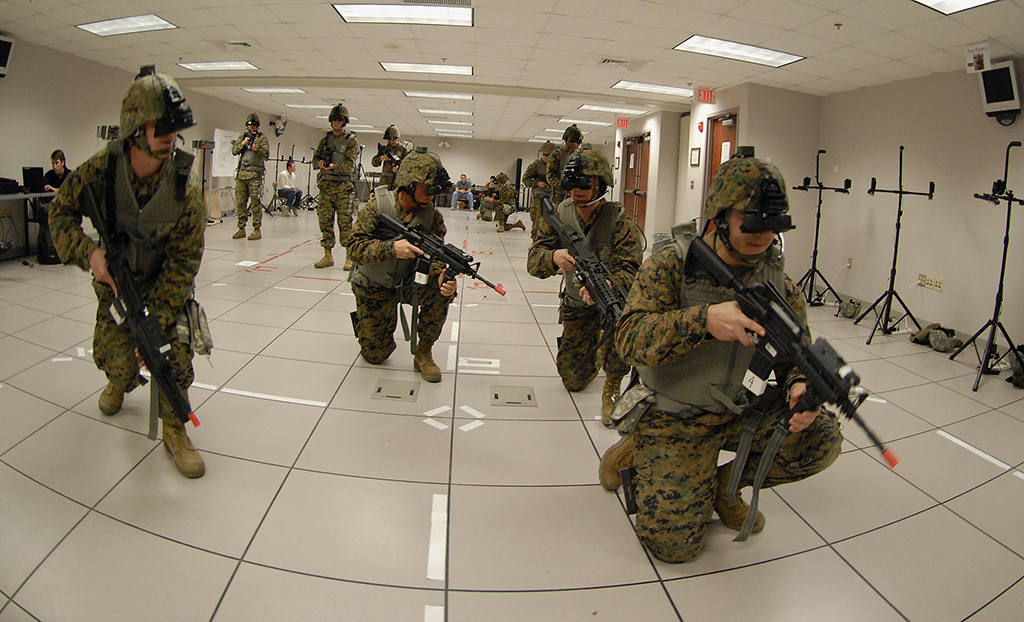
\includegraphics[width=10cm]{imagenes/vr_military}
	\caption{Marines de los Estados Unidos entrenando con el FITE (\textit{Future Immersive Training Environment}), un sistema de entrenamiento VR}
	\label{fig:vr_military}
\end{figure}

La verdadera importancia y utilidad de esto se muestra de dos formas muy claras: \textbf{facilidad de acceso}, requiriendo una serie de equipos mucho más al alcance y masificable; y \textbf{ahorro de recursos}, como podría ser el combustible de avión o la munición \cite{costeffective_vr}.

\subsection{Evolución y estado actual}

De hecho, la realidad virtual nunca había sido algo que se tuviese muy en cuenta a un nivel tecnológico hasta los últimos años, únicamente formando parte en conversaciones sobre futuros idílicos \cite{innovation_vr}. En la última década, en cambio, la evolución del hardware ha sido espectacular.

Las primeras gafas de realidad virtual como las conocemos ahora fueron el primer kit de desarrollo de Oculus, el cual tenía una resolución de 640x800 píxeles en cada ojo. A día de hoy, esta resolución ha llegado a cuadriplicarse (Figura \ref{fig:vr_resolution}). Además de resolución, otras muchas características también han avanzado, como el ángulo de visión, la tasa de refresco, uso inalámbrico, etcétera.

Aparte de las propias gafas, otros elementos físicos han tenido una evolución drástica, como por ejemplo mandos con una mayor optimización del uso de su batería o con seguimiento de posición de los dedos \cite{fingertracking}, nodos de seguimiento para colocar en diferentes puntos del cuerpo y capturar el movimiento de este, cámaras de captura de movimiento de la cara, y otros muchos elementos modulares que mejoran y amplían el uso de la realidad virtual.

\begin{figure}[H]
	\centering
	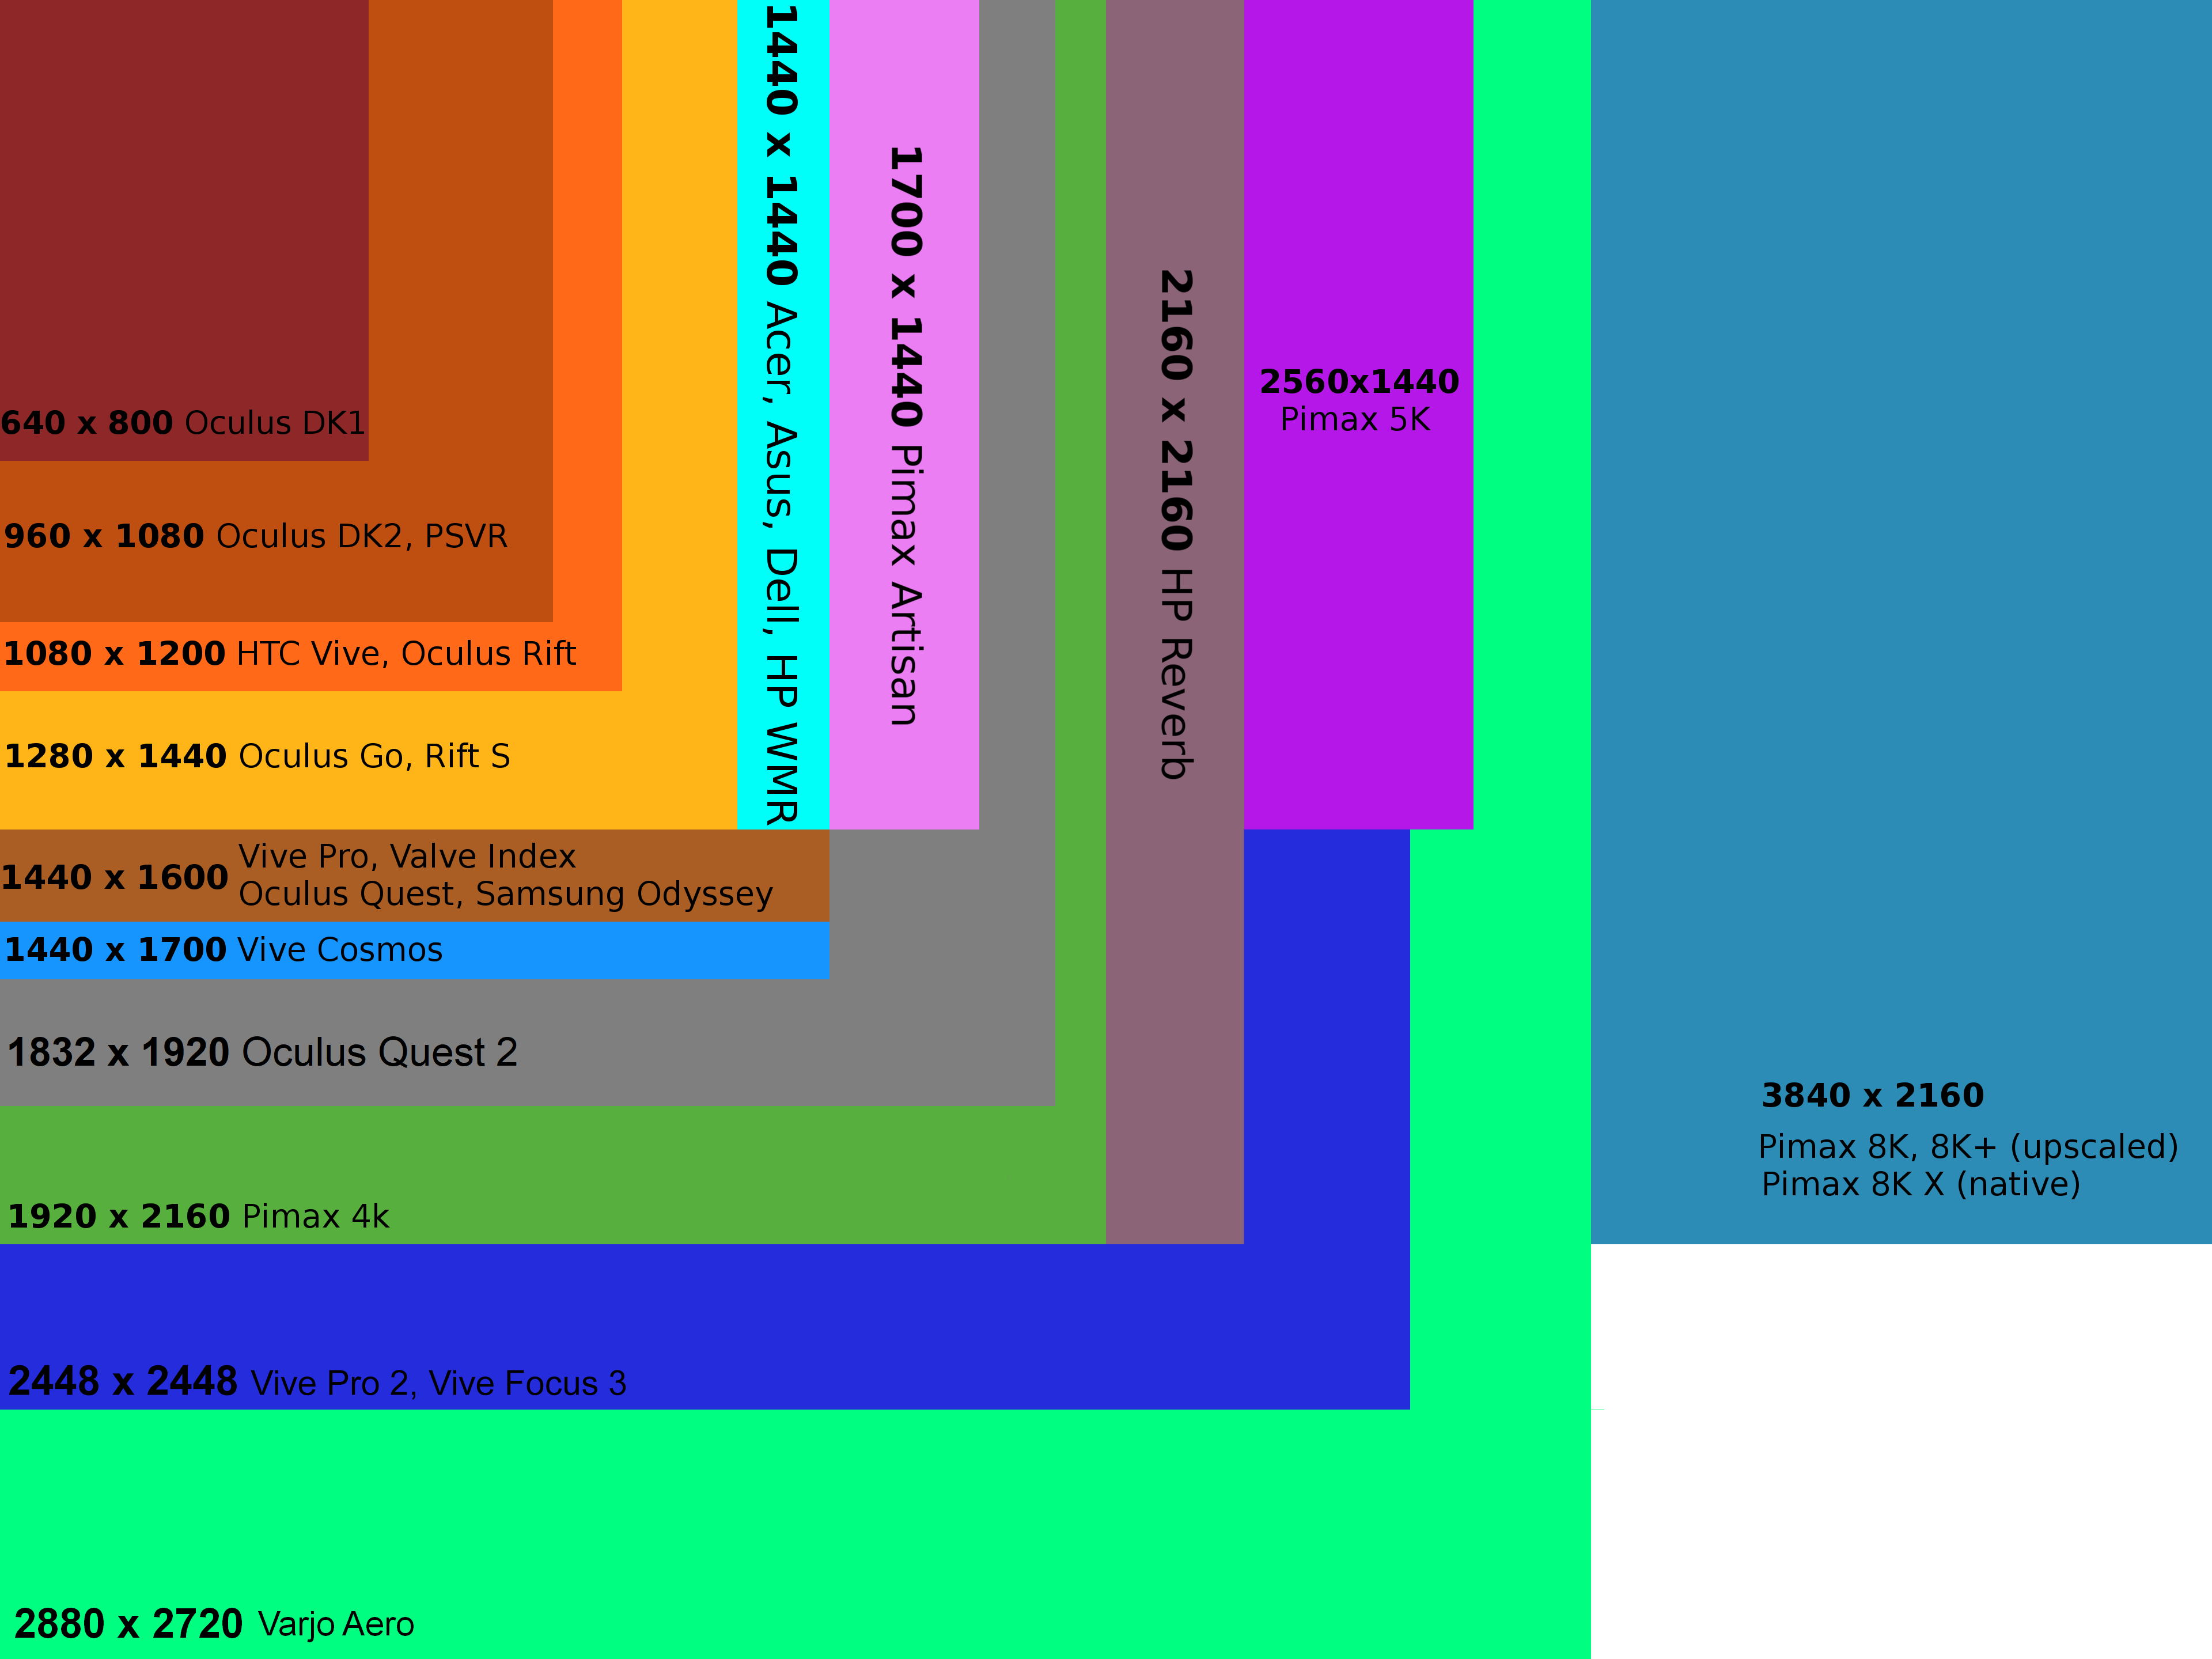
\includegraphics[width=10cm]{imagenes/vr_resolution}
	\caption{Tabla comparativa de la resolución por ojo de las gafas de realidad virtual más conocidas}
	\label{fig:vr_resolution}
\end{figure}

Además de simples mejoras físicas, la realidad virtual también se ha beneficiado de un gran \textbf{crecimiento en su comunidad}, tanto consumidores como desarrolladores de todo tipo debido a unas prestaciones cada vez más interesantes, lo que a su vez lleva a una mayor cantidad de productos, tanto software como hardware, junto a la demanda de estos \cite{vr_evolution}.

En lo que al desarrollo de aplicaciones respecta, las más avanzadas han sido creadas usando el motor gráfico \textbf{Unreal Engine 5} debido, entre otras razones, a su alto rendimiento y numerosas herramientas para el desarrollo de realidad virtual. Es por esto que se ha elegido para el proyecto en mano.

\section{Unreal}

Como ya se ha mencionado, Unreal es de los motores gráficos 3D más usados para el desarrollo de aplicaciones de realidad virtual, en concreto para las más especializadas. Esto se debe, entre otros factores, a las herramientas avanzadas que permiten aplicaciones imposibles de desarrollar en otros motores, además de un proceso más simplificado frente a estos \cite{unreal}.

En concreto, una biblioteca de Unreal lanzada recientemente, la cual permite \textbf{modificar la forma y colisión de los modelos en tiempo de ejecución a través de operaciones booleanas}, será clave en el desarrollo del proyecto, siendo la falta de una herramienta parecida la razón de que no existiese ninguna aplicación parecida hasta el momento.

\section{Escultura en mármol}

\subsection{Historia y características}

La escultura es uno de los artes más antiguos que existen, y en concreto, el mármol es de los materiales más usados para este. \textit{Venus de Milo} (100 a. C.), \textit{Laocoonte y sus hijos} (siglo I d. C.) (Figura \ref{fig:laocoonte_escultura}) o el \textit{David de Miguel Ángel} (1501-4 d. C.) son solo algunas de las obras más famosas esculpidas con esta técnica.

\begin{figure}[H]
	\centering
	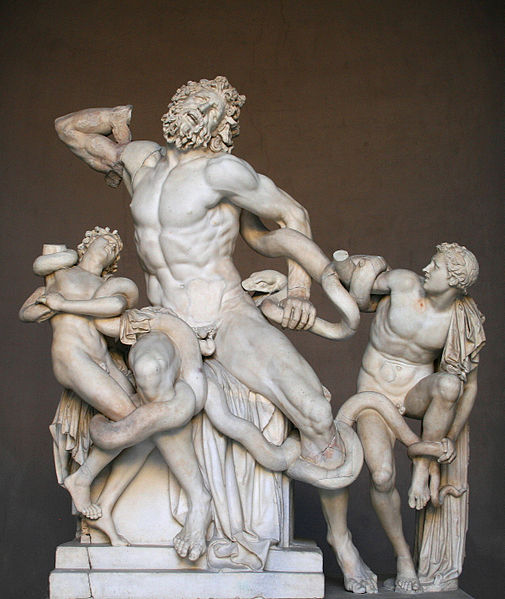
\includegraphics[width=6.5cm]{imagenes/laocoonte_escultura}
	\caption{\textit{Laocoonte y sus hijos}, también conocido como el Grupo del Laocoonte. Mármol copia de un original helenístico del 200 aC aproximadamente. Procedencia: Termas de Trajano, a principios de 1507.}
	\label{fig:laocoonte_escultura}
\end{figure}

El uso de mármol para la escultura se remonta a la Edad Antigua, y se ha utilizado tanto para relieves como para estatuaria. Desde entonces, ha sido un material apreciado por artistas debido a sus propiedades:

\begin{itemize}
	\item Fácil de trabajar y suave cuando se extrae.
	\item Adquiere dureza con la edad, lo que le da resistencia a la figura acabada.
	\item Variedad de tonos y patrones.
	\item Bajo índice de refracción de la luz, como la piel humana, lo que permite una apariencia humana.
	\item Grano más fino en comparación a otras piedras, lo que permite presentar detalles minuciosos.
\end{itemize}

Sin embargo, también existen una serie de inconvenientes. El mármol es muy pesado, más que otras piedras, además de más caro que estas. Otro inconveniente es que es más vulnerable a agrietarse que otros materiales como el bronce. También es menos resistente al clima que otras piedras como el granito, y absorbe con facilidad aceites como los de la piel, lo que puede causar manchas. \cite{sculpture_introduction}.

\subsection{Herramientas y técnicas}

Aunque se puede empezar la talla de forma directa, lo normal es esquematizar previamente la escultura a través de bocetos, tanto en dibujo como tallando versiones en miniatura con materiales baratos, para luego usarlos como guía para la figura final.

Una vez iniciado el proceso, se necesita una serie de herramientas para trabajar. Estas herramientas, aunque se han adaptado y mejorado a lo largo de la historia, son esencialmente las mismas, con el uso ocasional de utensilios más modernos para facilitar el proceso:

\begin{itemize}
	\item \textbf{Cincel}: La herramienta más importante en la escultura. Existen distintos tipos.
	\begin{itemize}
		\item \textbf{En punta}: Usado para quitar gran cantidad de material de un solo golpe, lo que permite llegar antes a la parte del mármol que conformará la propia escultura posteriormente. También existen cinceles de punta ancha con el mismo propósito.
		\item \textbf{De dientes}: Con múltiples dientes en la punta, que crean líneas paralelas. Se usa principalmente para refinar la forma dejada por el cincel en punta, eliminando irregularidades en la figura y permitiendo mayor comodidad y precisión al continuar.
		\item \textbf{Plano}: Como el nombre indica, la punta es plana, y sirve para tallar los detalles.
		\item \textbf{Redondo}: Lo mismo que el plano, pero con otro resultado en la textura.
	\end{itemize}
	\item \textbf{Martillo}: Con el que se golpea la parte roma del cincel para que la fuerza del golpe se concentre en la punta.
	\item \textbf{Bujarda}: Martillo con la cabeza recubierta de dientes. Se golpea directamente a la piedra con él para dejar formas rugosas.
	\item \textbf{Martillo neumático}: Martillo con mecanismo neumático para golpear reiteradas veces en un mismo punto. Se usa para lo mismo que el cincel en punta.
	\item \textbf{Radial}: Se usa para cavar líneas rectas de forma rápida. Una forma común, rápida y efectiva de quitar material inicial es hacer cortes paralelos con una radial para quitar el sobrante con martillo y cincel.
	\item \textbf{Limas, lijas, piedra pómez y otras}: Cualquier herramienta que sirva para pulir el resultado final.
\end{itemize}

Con todas estas herramientas se puede proceder a trabajar la piedra. Primero, se desbasta el material, es decir, se elimina todo el material muy exterior a lo necesario. Para esto se puede usar la radial, el martillo neumático o simplemente el cincel en punta. Conforme se progresa la tarea, se pasa a herramientas como el cincel de dientes para obtener la forma cruda de la escultura final, a la que luego se le añaden todos los detalles poco a poco con los cinceles planos y/o redondos. Finalmente, se pule y se limpia \cite{marble_techniques}.

\subsection{Complejidad y coste}

Como es de esperar, esta no es una práctica ni sencilla ni accesible. Acceso a todos los materiales, herramientas, espacio adaptado y necesario son algunos de los elementos necesarios para esculpir mármol. Además, mucha práctica e intentos fallidos son necesarios antes de obtener buenos resultados, lo cual puede llegar a ser muy frustrante, sobretodo cuando hace falta invertir tanto para siquiera iniciarse en el arte.

\section{Trabajos previos}

Existen muchas aplicaciones de realidad virtual que simulan prácticas del mundo real, ya sea de forma más ludificada y poco realista, como \textit{Cooking Simulator VR} (2021), o lo más cercano posible a la realidad, como el simulador de conducción \textit{Assetto Corsa} (2014), usado incluso por pilotos de carreras profesionales.

Por supuesto, también existen multitud de herramientas creativas que permiten dibujar, animar y, por supuesto, modelar en realidad virtual. \textit{SculptrVR} (2016) (Figura \ref{fig:sculptrvr}) o \textit{AnimVR} (2018) son algunos de los ejemplos de este tipo de aplicaciones, que permiten crear modelos en 3D o rodar películas de animación, respectivamente.

\setcounter{footnote}{0}

\begin{figure}[H]
	\centering
	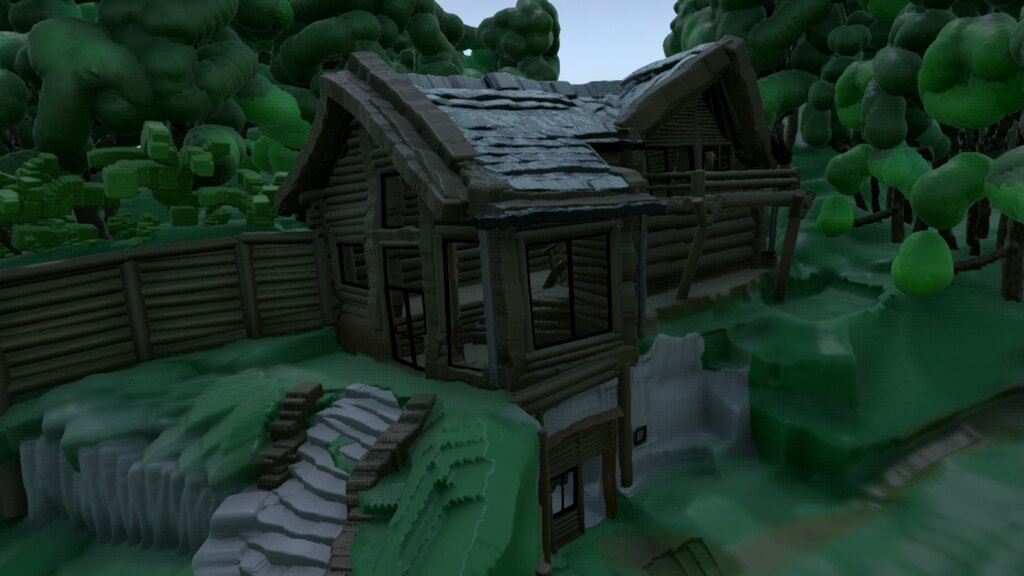
\includegraphics[width=10cm]{imagenes/sculptrvr}
	\caption[Captura de pantalla de una escena realizada en \textit{SculptrVR} por el usuario  topgunsi en Steam]{Captura de pantalla de una escena realizada en \textit{SculptrVR} por el usuario  topgunsi\protect\footnotemark[1]{} en Steam}
	\label{fig:sculptrvr}
\end{figure}

\footnotetext[1]{\url{https://steamcommunity.com/sharedfiles/filedetails/?id=1267529147}}

Sin embargo, generalmente, este tipo de aplicaciones no tratan de simular la realidad, sino que buscan \textbf{permitir formas de creatividad que no serían posibles fuera del mundo virtual}, como por ejemplo, dibujando objetos 3D en el aire.

\section{Motivación}

Por esta misma razón, la idea es desarrollar ChiselVR, un software para realidad virtual en el que, en lugar de crear esculturas a través de la adición como otras aplicaciones de modelaje, se crearían a través de \textbf{sustracción}, imitando el proceso de esculpir en mármol con sus correspondientes herramientas.

Por supuesto, esta es una forma más lenta y menos vistosa de modelar que la que ofrecen las demás aplicaciones, pero lo interesante reside en eso: \textbf{imitar la realidad} y permitir al usuario experimentar el proceso de esculpir de la forma tradicional sin tener que invertir en todo el material necesario para ello.

La aplicación final ofrecerá al usuario la posibilidad de iniciar un proyecto con un bloque de mármol que podrá esculpir a voluntad con las herramientas necesarias y esperadas para ello.

	\chapter{Descripción del problema}

En este capítulo se desarrollará el problema que se ha introducido en la sección anterior y que se quiere resolver, formulando los objetivos que se quieren alcanzar al final del proyecto.

\section{Problema a resolver}

La realidad virtual ofrece una cantidad de opciones para la creación de aplicaciones de entrenamiento de habilidades sin precedentes, lo cual la hace óptima para la creación de simuladores de todo aquello que requiera un alto coste en suministros y herramientas \cite{skill_training}. Este es el caso en el tema de esta aplicación, la escultura.

Esculpir a mármol directamente, sin conocimiento previo, es una idea muy desaconsejada por los expertos. El mármol es un material muy caro, por lo que lo recomendado es, para iniciarse, probar a esculpir en arcilla para adaptarse al proceso de tallar, seguido de intentar crear figuras con esteatita, un material bastante barato, y una vez listo, empezar a usar mármol \cite{rich1988materials}. La arcilla y la esteatita, sin embargo, son muy diferentes en comportamiento al mármol. Son materiales mucho más blandos, con la posibilidad de eliminar material incluso rasgando con un cuchillo. Por otro lado, cualquier otro material con una dureza y comportamiento mucho más parecidos al del mármol pasan a tener un precio que, aunque no necesariamente llega al nivel de este, sigue siendo considerablemente alto. Un simulador podría solucionar este problema.

Si se pretende ser lo más fiel posible a cómo sería realizar estas acciones en la vida real, se necesita, por una parte, conocer perfectamente el comportamiento físico real de aquello que se intenta imitar, y por otra parte, conseguir virtualizar este comportamiento. En el caso de la escultura, esto se traduce en conocer la dureza del mármol, la forma de quebrarse dependiendo de la fuerza y del tipo de herramienta, la importancia del ángulo al golpear, etcétera; y al mismo tiempo, por la parte virtual, cómo averiguar la fuerza y ángulo de impacto de los controladores por movimiento con el bloque, cómo eliminar una cantidad y forma realista del material a causa de este impacto, cómo conseguir un \textbf{rendimiento de la aplicación correcto y constante} pese al coste computacional necesario, y otras muchas cuestiones. Esto último será, si no el que más, de los factores más importantes a tener en cuenta durante el desarrollo de la aplicación.

Cabe añadir que desarrollar un simulador realista es una tarea ardua, donde es necesario un equipo amplio de desarrolladores. Es por eso que este proyecto apunta a construir las bases de dicho simulador, y servir así de \textbf{prueba de concepto} de lo que se puede lograr con la tecnología actual.

Por tanto, el problema principal a resolver en este trabajo es el de desarrollar un simulador que permita al usuario experimentar la experiencia de esculpir a mármol sin necesidad de invertir en todos los materiales y herramientas necesarios para ello. La aplicación también debe mantener un rendimiento bueno y constante, pese a la pesadez de las operaciones necesarias, ya que un rendimiento pobre podría resultar en malestar y náuseas en el usuario.

A continuación se describen los objetivos que busca alcanzar este proyecto en base a los problemas descritos. Se usarán posteriormente como medida para comprobar si el proyecto se ha finalizado correctamente.

\section{Objetivos}

Aquí se desglosan los objetivos específicos a alcanzar en este trabajo.

\begin{itemize}
	\item Diseñar y desarrollar una solución informática que permita, en realidad virtual, \textbf{tratar un cubo} como si fuese un bloque de mármol en la vida real.
	\item La solución permitirá al usuario \textbf{modificar e interactuar} con el cubo en tiempo real, eliminando material de este poco a poco.
	\item Implementar distintas \textbf{herramientas} que imiten el comportamiento de sus contrapartes reales y permitan al usuario interactuar de distintas formas.
	\item La solución debe tener una navegación y unos controles \textbf{intuitivos}, que permitan a los usuarios entender el funcionamiento de la aplicación con facilidad.
	\item Añadir una serie de efectos y presentar los elementos en pantalla de tal forma que la experiencia sea más \textbf{inmersiva} para el usuario.
	\item La solución debe estar \textbf{optimizada} y mantener un rendimiento adecuado en la ejecución, algo esencial en cualquier aplicación 3D y específicamente en aplicaciones de realidad virtual.
\end{itemize}

	\chapter{Estado del arte}

En este capítulo se introducirán varios de los conceptos clave que se mencionarán a lo largo del trabajo, definiéndolos y detallando su estado actual respecto al ámbito de este proyecto. Con esto se facilitará el entendimiento de todo aquello que se explique en los capítulos posteriores.

El capítulo se compone de dos partes diferenciadas. Primero, se describirán distintos aspectos y tecnologías relativos al dominio del problema como el estándar actual de las aplicaciones de realidad virtual, las operaciones booleanas y las colisiones en entornos 3D interactuables y su coste computacional. Después, se analizarán otros trabajos que tengan el objetivo final de esculpir en realidad virtual, además de proyectos que, aunque no tengan el mismo objetivo, usen las mismas herramientas que esta aplicación.

\section{Dominio del problema}

Aquí se discutirán los conceptos más importantes en relación al dominio del problema para poder entender posteriormente el resto del trabajo: estado actual de las aplicaciones en realidad virtual, estándares de calidad y salud; y las operaciones booleanas, sus usos y las opciones que nos ofrece al combinarlas con hardware y software modernos, además del conflicto que suponen al usarlo en tiempo real con simulación de colisiones.

\subsection{Aplicaciones de Realidad Virtual}

En el capítulo 1 ya se ha explicado qué es la realidad virtual, pero para reiterar, es el campo de la informática gráfica que estudia la presentación e interacción con el usuario de tal forma que este se sienta trasladado a, como el nombre indica, otra realidad.

Para conseguir esto, las aplicaciones de realidad virtual deben cumplir una serie de estándares que cumplen, principalmente, dos funciones: mantener la \textbf{inmersión} del usuario y evitar el malestar físico y el peligro (\textbf{seguridad})\cite{vrstandard}. Estos estándares, debido a lo reciente que es el campo de estudio al que pertenecen, han ido cambiando considerablemente, pero se han ido asentando en años recientes. Se ahondará en las funciones mencionadas a continuación.

Primero, la inmersión. Como es de esperar, en un campo como la realidad virtual una de las principales preocupaciones es conseguir que el usuario, dentro de lo seguro y posible, se sienta dentro de la aplicación. Para conseguir esto, se deben seguir una serie de pautas. Primero, cualquier tipo de interacción con la aplicación debe ser, en la medida de lo posible, \textbf{intuitiva}. Esto conlleva usar esquemas de control que reflejen el comportamiento real de lo que se va a hacer. Un ejemplo de esto sería, al usar una pistola, que el botón de disparar fuese el gatillo del mando y no cualquier otro, o traído al ámbito de este proyecto, que un cincel y un martillo no usen en ningún momento control por botones y que únicamente sea necesario moverlos como se haría en la vida real para que funcionen. Otros elementos necesarios para una correcta inmersión es el uso de \textbf{efectos visuales y sonoros y feedback háptico} que vendan de forma correcta la acción que se está realizando. Usando los mismos ejemplos de antes, una pistola tiene que hacer un sonido concreto que lo distinga de otras armas de fuego, y un martillo golpeando un cincel producirá un sonido y una vibración mayor o menos dependiendo de la fuerza con la que se golpee.

Respecto a la seguridad y bienestar del usuario, muchas veces entra en conflicto con la inmersión. Un buen ejemplo de esto es el sistema de locomoción: aunque un movimiento libre usando el \textit{joystick} resulte más interesante y atractivo, en realidad lo más recomendado es usar un sistema de \textbf{teletransportes} a través del cual el usuario puede apuntar a una localización y desplazarse automáticamente a esta. Esto se debe a que, parecido a la sensación que puede dar ir por un terreno accidentado en un vehículo, la locomoción continua es causante de náuseas y mareos. Por esta razón, con los años se ha ido adoptando más el permitir al usuario elegir entre un sistema de locomoción y otro, generalmente estableciendo el método por teletransportes como el predeterminado (Figura \ref{fig:plantillaunreal}).

\begin{figure}[H]
	\centering
	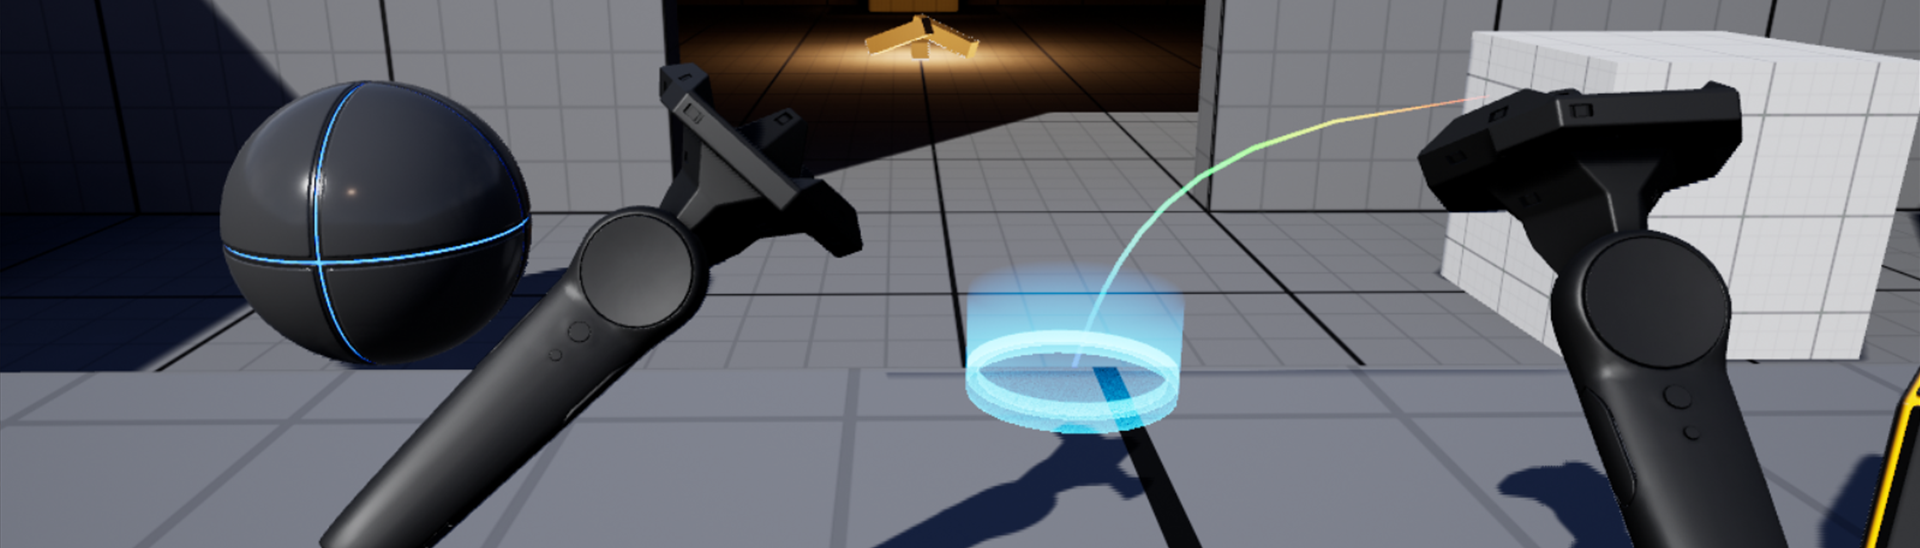
\includegraphics[width=10cm]{imagenes/plantillaunreal}
	\caption{Imagen extraída de la documentación oficial de la plantilla de proyecto VR de Unreal Engine. Se puede observar la locomoción por teletransporte siendo usada}
	\label{fig:plantillaunreal}
\end{figure}

Otro elemento importante a tener en cuenta al desarrollar con el bienestar del usuario en mente es el rendimiento de la aplicación, como ya se ha mencionado previamente. Generalmente, el ojo humano es capaz de distinguir cambios de luz y movimiento aproximadamente 60 veces por segundo, razón por la que se ha usado como estándar en muchas industrias a lo largo del tiempo. Sin embargo, esta capacidad no es estática, ya que el ojo está preparado para captar \textbf{frecuencias mucho más altas} en momentos puntuales, como cuando se perciben movimientos rápidos o se presta mucha atención en una acción \cite{refresh_rate}. En pantallas convencionales, una tasa de refresco de 60 fotogramas por segundo es más que suficiente, pero en realidad virtual es necesario alcanzar una tasa cuanto más alta mejor, pues al privar a la visión de la fluidez que percibe en el mundo real, puede llegar a causar en el usuario molestias como las mencionadas en el problema de la locomoción. Para poder alcanzar estas tasas de refresco es de gran importancia, más que en otros campos de la informática gráfica, tener muy en cuenta el rendimiento y la optimización de la aplicación.

Afortunadamente, muchos motores gráficos ofrecen plantillas a los desarrolladores para facilitar la implementación y correcto seguimiento de estos estándares. En concreto, Unreal Engine, el motor que se usará en este proyecto, ofrece en su plantilla un sistema de locomoción ya implementado y documentado con la posibilidad de ser manipulado como se desee; diferentes objetos interactuables como pistolas de los cuales partir para crear herramientas que pueda usar el usuario posteriormente; y opciones para el uso de tecnologías como FSR (\textit{Fidelity Super Resolution} de AMD), que permiten \textbf{renderizar la imagen a una calidad menor sin que se note diferencia en el resultado}, de forma que se obtiene mejor rendimiento y una tasa de refresco más alta y estable.

\subsection{Operaciones booleanas en geometría}

Para comprender las operaciones booleanas en el dominio de los entornos 3D, primero es necesario comprender en qué consisten las operaciones booleanas convencionales. Las operaciones booleanas son un conjunto de operaciones lógicas fundamentales para manipular valores binarios. Estas operaciones incluyen la negación, NOT, que cambia el valor de cualquier expresión a su contrario (es decir, de verdadero a falso y viceversa); la conjunción, AND, que devuelve verdadero únicamente si todos los valores de entrada son verdaderos; y la disyunción, OR, que devuelve verdadero si cualquiera de los valores de entrada es verdadero. Aparte de estas operaciones, existen otras derivadas de ellas las cuales no son tan relevantes para el dominio de la geometría.

Ahora, al aplicar las operaciones booleanas en la geometría, el funcionamiento es el mismo solo que en lugar de valores binarios, los datos que se manipulan son \textbf{figuras poligonales}. De esta forma, partiendo de dos objetos 3D distintos, se pueden conseguir resultados como por ejemplo el area de la primera figura sin la de la segunda, una suma de las dos o la intersección entre ambas (Figura \ref{fig:operacionesbooleanas}). En relación con las operaciones booleanas convencionales, la operación NOT se sustituye por una resta, es decir, que \textbf{la figura resultante sea la parte de la primera que \textit{no} coincide con la segunda}.

\begin{figure}[H]
	\centering
	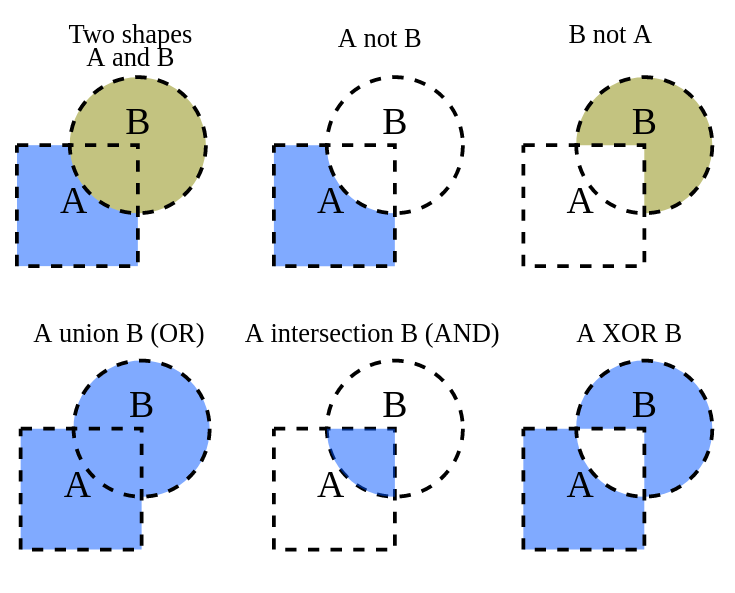
\includegraphics[width=10cm]{imagenes/operacionesbooleanas}
	\caption{Diferentes operaciones booleanas representadas en un espacio 2D}
	\label{fig:operacionesbooleanas}
\end{figure}

Incluso después de múltiples innovaciones en algoritmos para calcular las figuras resultantes de las operaciones booleanas, siguen teniendo un \textbf{alto coste computacional} y por tanto su uso siempre se ha visto reducido a aplicaciones donde el rendimiento no es de máxima prioridad \cite{boolean_operations}. Por esta razón, rara vez se ha usado en un medio interactivo como simuladores o videojuegos, menos aún en algo como realidad virtual, donde el rendimiento es clave. Pero recientemente, existen herramientas experimentales que permiten su viabilidad en este tipo de tareas.

En 2022, Epic Games lanzó un plugin experimental llamado \textbf{Geometry Script} para la última versión de su motor gráfico, Unreal Engine 5\footnote{\url{https://docs.unrealengine.com/5.0/en-US/geometry-script-users-guide/}}. Este plugin, entre otras muchas nuevas opciones de edición de generación y edición de mallas 3D, permite usar dentro de \textit{Blueprints} (equivalente en este motor gráfico a las clases en la programación por objetos) funciones normalmente solo accesibles en editores y aplicaciones de modelaje como Blender o Maya. Esto permite usar dichas funciones en tiempo de ejecución, es decir, se podrá implementar en una aplicación funcional y que el usuario final pueda usarlas para interactuar con esta. Aunque técnicamente esto era antes posible con plugins desarrollados por terceros o usando otras herramientas de gráficos 3D en base a código (como Three.js), este plugin es pionero en el uso de estas funciones de forma viable, pues hasta ahora \textbf{ninguna de estas opciones ofrecía una solución suficientemente optimizada para una aplicación de interacción en tiempo real}.

Algo relevante sobre las operaciones booleanas en el contexto de este proyecto es su relación con la simulación de colisiones. Primero, cabe destacar un dato importante sobre las colisiones: en videojuegos, simuladores y otras aplicaciones similares, \textbf{las colisiones son el factor con más coste computacional de todos}, incluso por encima de calidad gráfica y efectos visuales como las luces \cite{collisions}. Esto se debe a la necesidad de realizar una gran cantidad de comprobaciones por segundo en diferentes puntos a la vez. Por esta razón, donde más se trabaja para optimizar el coste computacional es en las colisiones, usando técnicas como la simplificación de la geometría usada para la lógica de colisiones (Figura \ref{fig:colisiones}).

\begin{figure}[H]
	\centering
	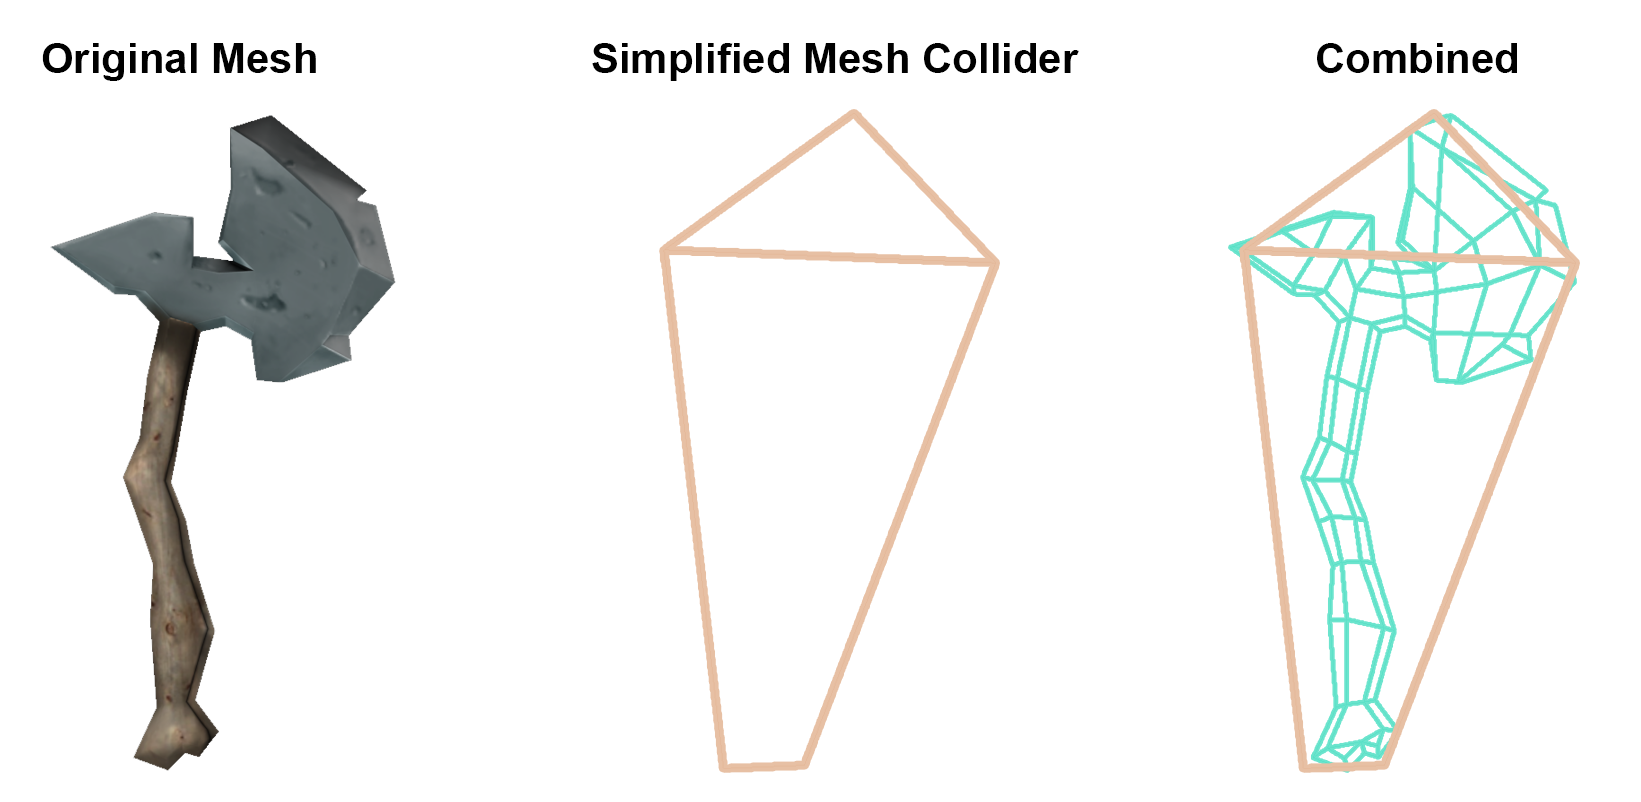
\includegraphics[width=10cm]{imagenes/colisiones}
	\caption{Comparación de la malla visual con la malla de colisión}
	\label{fig:colisiones}
\end{figure}

La razón por la que es relevante en relación a las operaciones booleanas es aparente: si se modifica la malla visual en tiempo de ejecución, también se debe modificar la malla de colisiones en caso de querer usarse en la simulación de estas. Si se deja la malla de colisiones igual que la visual, su simple existencia supone un altísimo coste computacional, mientras que si se simplifica la malla después de realizar la operación, el tiempo para realizar la operación es aún más notable, lo cual no es deseable. De hecho, en el contexto de ChiselVR, sería necesario que \textbf{ambas mallas sean iguales}, lo cual, como se ha mencionado, es algo difícil de conseguir. Por suerte, combinando el alto rendimiento de Unreal Engine 5 con hardware moderno, \textbf{ahora es algo posible}, y por tanto será lo que se usará para el desarrollo de este proyecto.

\section{Trabajos relacionados}

Aquí se discutirán otros trabajos y proyectos relacionados con la simulación de esculturas y modelaje en realidad virtual, además de otros proyectos que usan la misma tecnología que usará ChiselVR.

\subsection{Escultura en Realidad Virtual}

Como se ha mencionado en el capítulo 1, existe una gran cantidad de herramientas que permiten al usuario expresar su creatividad en realidad virtual. Entre ellas, efectivamente, existen muchas dedicadas a la creación de esculturas y otro tipo de arte tridimensional, pero con un enfoque claramente distinto al de ChiselVR: más a través de la adición de material que en la sustracción de este, y mucho más \textbf{enfocados en el resultado final} y no tanto en el arte que conlleva el proceso a este. A continuación, se profundizará en una de las aplicaciones más populares de este sector para entender mejor esta diferencia:

\subsubsection*{\textit{SculptrVR} (2016)}

SculptrVR\footnote{\url{https://www.sculptrvr.com/}} es una aplicación de modelado en realidad virtual con una gran cantidad de opciones a la disposición del usuario. Entre las herramientas más destacadas se incluyen:

\begin{itemize}
	\item Pinceles con distintos tamaños, formas y estilos para dibujar formas geométricas en el aire.
	\item Herramientas de manipulación varias, con las que modificar de diversas formas las figuras ya creadas y así realizar ajustes más precisos.
	\item Pinturas y texturas, para cambiar el aspecto de las figuras.
	\item Opciones de duplicación y simetría para facilitar la creación de este tipo de figuras.
	\item Herramientas de paisaje y escala, que permiten crear no solo objetos individuales, sino escenas completas.
	\item Funcionalidades colaborativas, con las que múltiples usuarios pueden participar al mismo tiempo en la creación de una escena.
	\item Herramientas para exportar los proyectos finalizados
\end{itemize}

Por todas las opciones listadas, su accesibilidad y su disponibilidad en múltiples plataformas, SculptrVR es de las aplicaciones más populares para la creación de objetos 3D en entornos de realidad virtual. Sin embargo, \textbf{esta aplicación no es un simulador, ni pretende serlo}: las figuras creadas flotan y no interactuan unas con otras. No bloquean el paso de las herramientas cuando estas colisionan contra su superficie, ni se parten al recibir un impacto (Figura \ref{fig:sculptvr2}).

\begin{figure}[H]
	\centering
	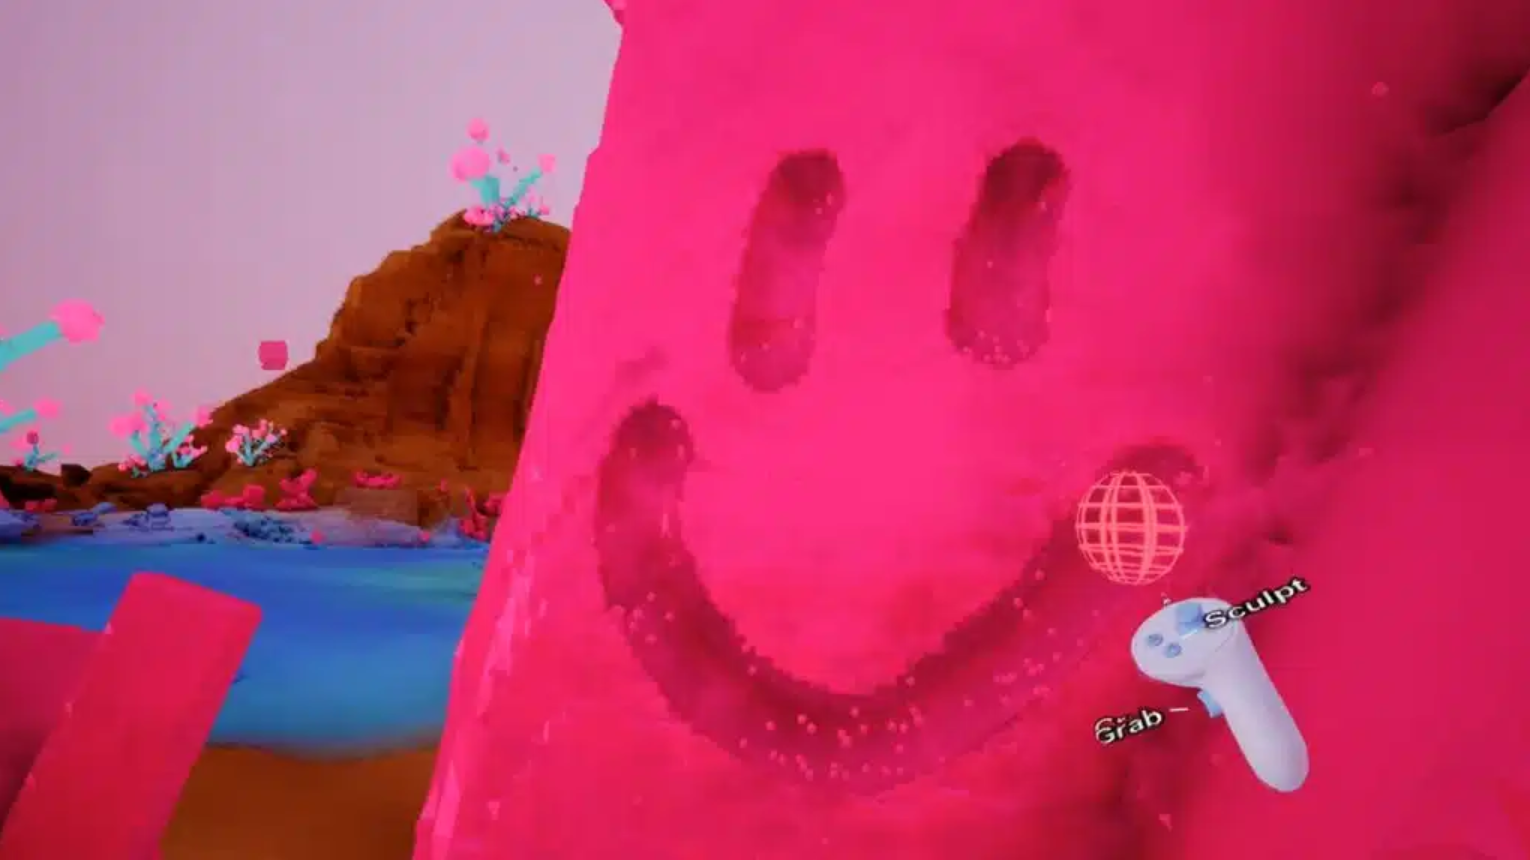
\includegraphics[width=10cm]{imagenes/sculptrvr2}
	\caption{Herramienta de tallado en SculptrVR. Aunque se elimine material de la figura, no simula la acción real de esculpido, sino que simplemente se va eliminando el material dentro del área marcada.}
	\label{fig:sculptvr2}
\end{figure}

Esto es por un lado, por supuesto, el funcionamiento deseado de la aplicación, pues su objetivo es facilitar la creatividad del usuario sin ninguna limitación, pero por otro lado es precisamente donde se distingue de este proyecto, ChiselVR, ya que el objetivo de este es simular la experiencia real de esculpir, con su dificultad y la pesada pero relajante monotonía que esta conlleva.

\subsection{Proyectos con Geometry Script}

El lanzamiento al público del plugin Geometry Script es considerablemente reciente, y aún no existen proyectos estables que lo usen. De hecho, el propio motor no lo permite, ya que Unreal Engine no tiene en cuenta elementos y funciones experimentales (como es el caso de Geometry Script) al empaquetar proyectos, es decir, crear una aplicación ejecutable sin la necesidad de usar el motor gráfico para ello.

Sin embargo, sí que existen desarrolladores trabajando en investigar las posibilidades que ofrece este plugin, y a continuación se mostrarán algunos de sus proyectos.

Primero, cabe mencionar a Ryan Schmidt, uno de los desarrolladores detrás de Geometry Script, que ha estado los últimos meses publicando tutoriales, explicaciones y experimentos usando este plugin\footnote{\url{https://www.youtube.com/@RyanSchmidtEpic/featured}}. En sus vídeos, se muestran ejemplos de uso de muchas de las funciones disponibles, tanto de forma independiente como combinándolas entre sí. Las publicaciones de este desarrollador son tan valiosas para comprender Geometry Script como la propia documentación del plugin.

Otro proyecto que muestra el potencial de Geometry Script es el experimento combinando las operaciones booleanas con proyectiles de parte del usuario de \textit{YouTube} Quantaxy\footnote{\url{https://www.youtube.com/@quantaxy}}. En este proyecto, Quantaxy usa las operaciones booleanas para crear \textbf{impactos de bala} en la pared, llegando incluso a perforar a través de esta. En resumidas cuentas, la lógica usada es:

\begin{itemize}
	\item Detectar el punto de impacto del proyectil en la pared.
	\item Calcular la velocidad del proyectil en el momento de impacto.
	\item Combinar ambos datos para calcular la profundidad del impacto en la pared.
	\item Realizar la operación booleana para eliminar material de la pared.
\end{itemize}

De esta forma, es posible crear la ilusión de que es el propio proyectil el que rompe la pared, y no a través de roturas procedurales o vóxeles (es decir, que la pared fuese compuesta por multitud de cubos pequeños en lugar de un único bloque) como se ha hecho tradicionalmente, sino con un golpe exacto y realista (Figura \ref{fig:booleans_at_runtime}). Es por eso que este proyecto, que no tiene ninguna relación con la escultura, sirvió de inspiración para ChiselVR: al esculpir, aproximaciones como en los métodos tradicionales no sirven; se necesita algo más \textbf{exacto}, y eso es exactamente lo que permite Geometry Script.

\begin{figure}[H]
	\centering
	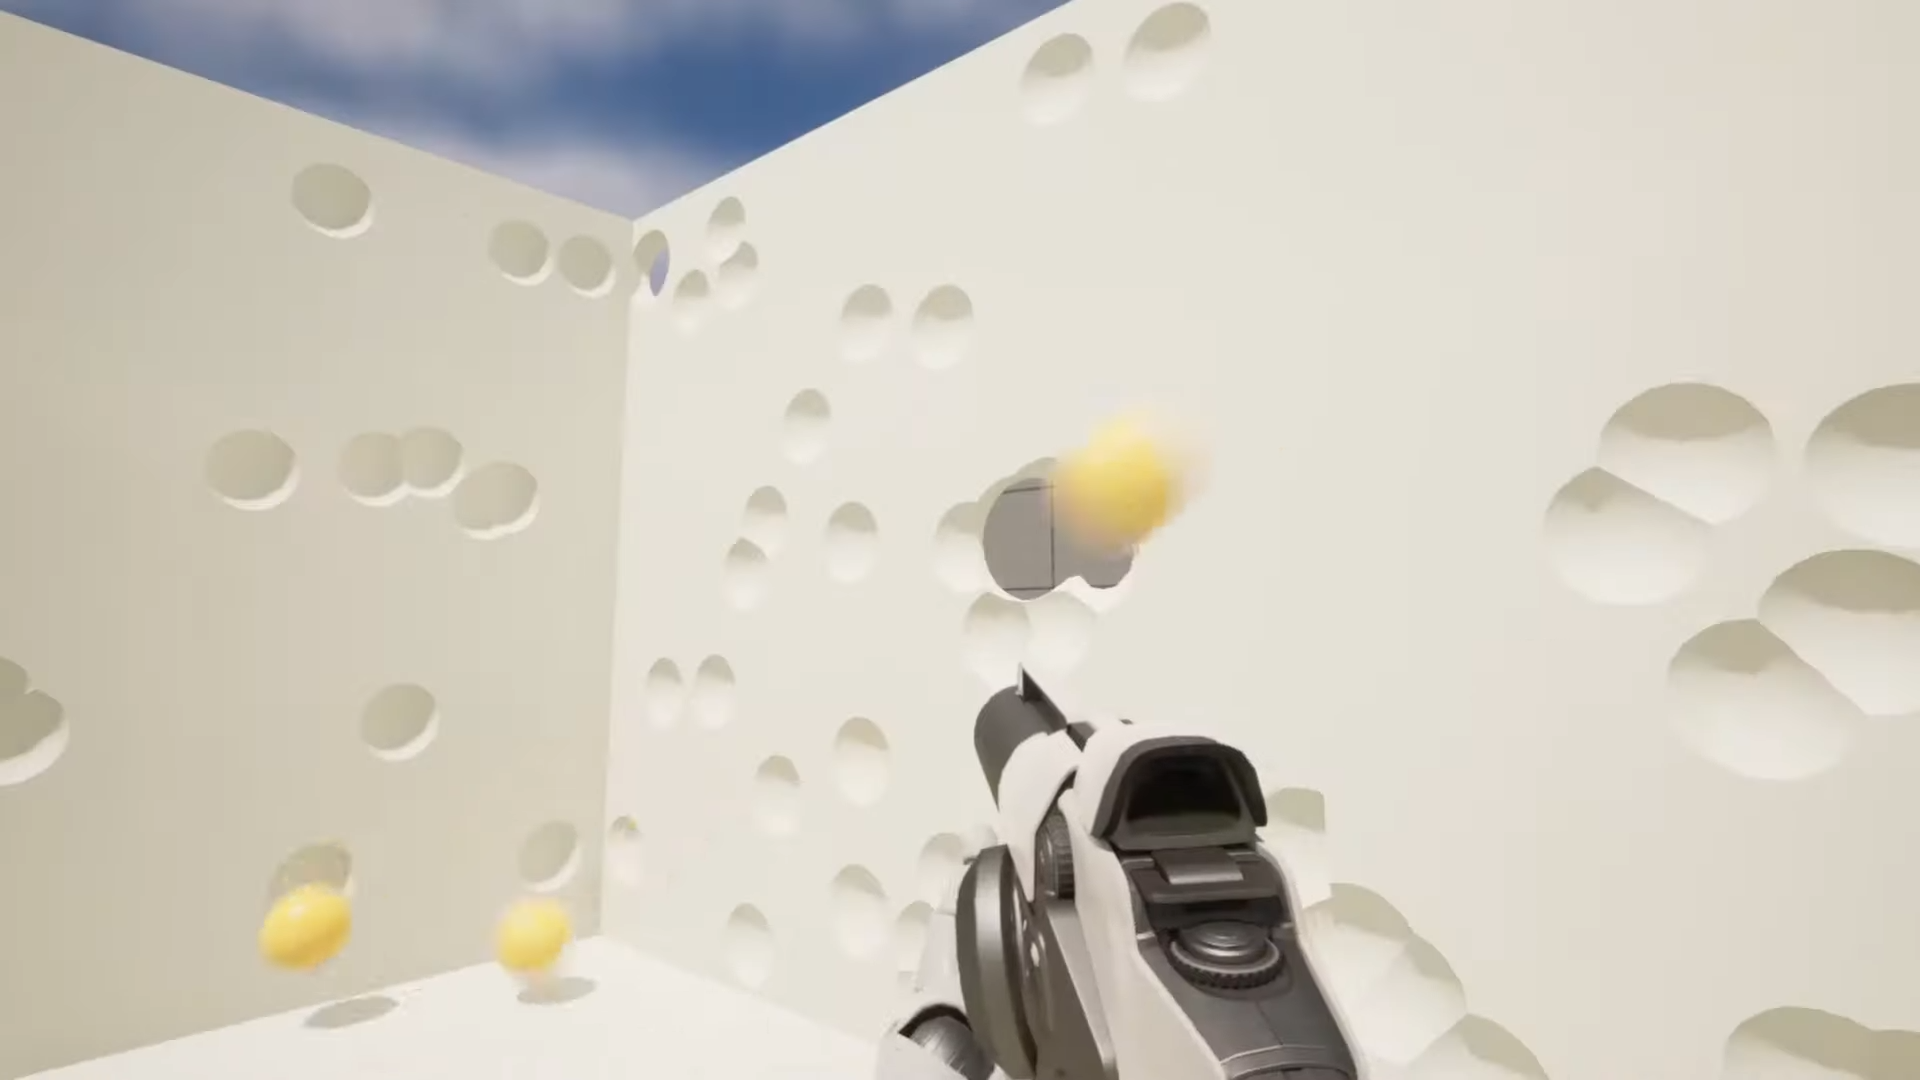
\includegraphics[width=10cm]{imagenes/booleans_at_runtime}
	\caption{Captura de pantalla del proyecto de Quantaxy en ejecución. Se pueden ver múltiples impactos en las paredes, llegando incluso a atravesar una de ellas.}
	\label{fig:booleans_at_runtime}
\end{figure}
	
	\chapter{Planificación}

En este capítulo se abarcarán todas las cuestiones relacionadas con la planificación del proyecto: organización previa, metodologías, planificación y control de calidad. Estos factores se detallarán a continuación, empezando por la metodología utilizada.

\section{Metodología utilizada}

El software puede tomar muchas formas. Desde programas sencillos para automatizar una tarea simple, hasta videojuegos con presupuestos multimillonarios o editores de vídeo usados en la producción de películas.  Y conforme crece la escala de un software, la complejidad para gestionar todo crece exponencialmente, junto con la necesidad de hacerlo.

Tradicionalmente, esta gestión del desarrollo se hacía detallando unos objetivos claros y fijos al principio del desarrollo, y de los cuales se esperaba su finalización al final del proyecto. Esto, como cabe esperar, era una aproximación problemática, pues esta visión estática fallaba en predecir la espontaneidad de los problemas que pueden surgir a lo largo del desarrollo. Entran entonces las \textbf{metodologías de desarrollo ágil}, las cuales, como bien su nombre indican, son más versátiles a la hora de encarar los problemas y cambios a lo largo del desarrollo. Existen distintas metodologías ágiles, pero para este proyecto se ha escogido \textbf{SCRUM} \cite{scrum}, una metodología perfecta para equipos pequeños o, como es el caso, individuales.

La metodología SCRUM se compone de distintos elementos, siendo los más relevantes para el proyecto los siguientes:

\begin{itemize}
    \item \textbf{Backlog del producto}. Una lista priorizada de todas las funcionalidades, requisitos y cambios potenciales en el producto.
    \item \textbf{Sprint}. Es un período de tiempo fijo (de una semana en este proyecto) durante el cual se desarrolla un incremento de producto potencialmente entregable.
    \item \textbf{Backlog del sprint}. Una selección de elementos del backlog del producto que se comprometen a desarrollar en el sprint actual.
    \item \textbf{Incremento}. El conjunto de elementos del backlog del producto completados durante el sprint y que están listos para su entrega.
\end{itemize}

En este proyecto se han omitido los diferentes tipos de reuniones que también forman parte de la metodología SCRUM debido a la ausencia de un equipo con múltiples desarrolladores, en cambio se han realizado actualizaciones periódicas con el tutor para discutir el estado actual y futuro del proyecto (sustituyendo así el Scrum Diario, una reunión diaria corta donde los miembros del equipo comparten lo que hicieron el día anterior, lo que planean hacer ese día y si enfrentan algún obstáculo).

\section{Historias de usuario}

Para la descripción de los requisitos que debe cumplir ChiselVR, se ha empleado el método de historias de usuario, las cuales consisten en descripciones breves y simples de funcionalidades específicas que el producto debe proporcionar desde la perspectiva del usuario final. Se han redactado durante el primer sprint del desarrollo, y es de donde surgen las tareas que posteriormente se gestionarán en el desarrollo.

La redacción de las historias de usuario requiere la creación de uno o varios perfiles que reflejen los tipos de usuarios que usarán la aplicación. En este caso, se distingue un único perfil de usuario: aquel del consumidor medio de realidad virtual, el cual busca contenido que solo pueda experimentar con controles por movimiento y un visor en la cabeza. Este usuario no tiene por qué tener más conocimiento técnico que el de navegar por los menús de su sistema de realidad virtual, y podría incluso no tenerlos y ser simplemente el invitado de aquel que sí los tiene y le está enseñando cómo es la realidad virtual.

También se ha planteado la inclusión del usuario creador de contenido, sin embargo, como ya se ha discutido anteriormente, la naturaleza de este proyecto es más cercana al simulador que al editor gráfico, por lo que no existe razón lógica por la que un usuario de este tipo optaría por ChiselVR para su objetivo.

A partir del perfil de usuario definido se obtendrán los \textit{customer journeys}, los cuales describen el proceso que lleva a un hipotético usuario (el cual entra dentro de los perfiles que se hayan detallado anteriormente) a interactuar con el producto. Su objetivo es, al ponerse en los pies del usuario final, entender mejor las necesidades de este y reflejarlas en las historias de usuario. Los \textit{journeys} ideados son los siguientes:

\begin{itemize}
    \item \textbf{J-1, Óscar Llorens}. Joven de 21 años aficionado de la tecnología. Se compró recientemente el kit de realidad virtual Meta Quest 2, y está buscando aplicaciones de todo tipo para estrenarlas. En su búsqueda, entra en la sección \textit{Engage your palette} de la tienda online, donde se encuentran todas las aplicaciones sobre creatividad. Añade unas cuantas a la lista de deseados, entre ellas SculptrVR y ChiselVR, con las que espera experimentar el proceso de esculpir una piedra. Primero usa SculptrVR, pero ve que no es lo que esperaba. Después, abre ChiselVR y descubre que, esta vez sí, puede esculpir golpeando la pieza, eliminando el material poco a poco. Al ver lo relajante y directo que es el funcionamiento de la aplicación, decide que será una de las aplicaciones que enseñará a sus padres cuando vaya a mostrarles cómo es la realidad virtual.
    \item \textbf{J-2, César Manchón}. Hombre de 46 años, emprendedor interesado en realidad virtual como sector de negocio. Cada cierto tiempo, investiga sobre aplicaciones recién lanzadas para ver cuáles tienen potencial. Entre estas ve ChiselVR, y como César también es aficionado del arte, decide echarle un ojo. Al crear una nueva escena y probar un rato el martillo y el cincel, ve que la premisa tiene potencial, pero se pregunta si tiene algo más. Al pulsar el botón del menú, descubre que tiene otra herramienta más, una sierra radial, y que funciona exactamente como esperaba. Cuando acaba de usarla, ve que por ahora ya no hay más herramientas, pero se pone a pensar en las posibilidades que hay si sigue el desarrollo. Interesado, decide mantener un ojo en la aplicación para posibles futuras actualizaciones.
    \item \textbf{J-3, Ana Torrecilla}. Mujer de 57 años, madre de Óscar Llorens. Ana no toca muchos aparatos electrónicos más allá de su teléfono y el ordenador que usa para el trabajo, pero su hijo insiste en enseñarle la realidad virtual. La primera aplicación que le muestra es ChiselVR. Nada más ponerse el visor, se ve a sí misma con un cincel y un martillo en las manos, y con un bloque delante. Hace el gesto de esculpir, y se alegra al ver que funciona, pero se siente algo molesta: Ana es zurda, y en la posición actual en la que tiene las manos se le hace incómodo. Óscar le dice que se mantenga quieta un segundo, y procede a darle al menú por ella. Después le pregunta a su madre si ve la opción de cambiar manos, y que si la ve que le apunte y la seleccione. Ana le da, y ahora cada herramienta está en la mano contraria a la que estaba antes, con lo que procede a estar unos minutos jugando con el mármol hasta que se cansa.
\end{itemize}

Una vez descritos los \textit{costumer journeys}, se obtiene un mayor entendimiento de las necesidades de los usuarios, por lo que nos es posible desarrollar las historias de usuario. Estas se compondrán de nombre, descripción, estimación en horas del tiempo necesario para cumplirlas, prioridad, dependencias a otras historias de usuario y pruebas de aceptación.

\begin{table}[H]
	\begin{center}
		\begin{tabular} {l|c|l}
			\hline
			CH-1 & \multicolumn{2}{c}{Escena navegable} \\ \noalign{\hrule height 1pt}
			\multicolumn{3}{l}{Descripción} \\ \hline
			\multicolumn{3}{p{12cm}}{Como usuario quiero poder iniciar una escena por la que puedo moverme en realidad virtual.} \\ \noalign{\hrule height 1pt}
			\multicolumn{2}{l|}{Estimación} & 5 \\ \hline
			\multicolumn{2}{l|}{Prioridad} & ALTA \\ \hline
			\multicolumn{2}{l|}{Dependencias} & - \\ \noalign{\hrule height 1pt}
			\multicolumn{3}{l}{Pruebas de aceptación} \\ \hline
			\multicolumn{3}{p{12cm}}{ - Se puede entrar en la escena y moverse por ella.} \\
            \multicolumn{3}{p{12cm}}{ - No se puede navegar por terreno ocupado por otros objetos.} \\ \hline
		\end{tabular}
	\end{center}
	\caption{Historia de usuario - Escena navegable}
	\label{tab:hu_escena_navegable}
\end{table}

\begin{table}[H]
	\begin{center}
		\begin{tabular} {l|c|l}
			\hline
			CH-2 & \multicolumn{2}{c}{Bloque de mármol} \\ \noalign{\hrule height 1pt}
			\multicolumn{3}{l}{Descripción} \\ \hline
			\multicolumn{3}{p{12cm}}{Como usuario quiero disponer de un bloque con el que interactuar de distintas formas para poder modificarlo.} \\ \noalign{\hrule height 1pt}
			\multicolumn{2}{l|}{Estimación} & 10 \\ \hline
			\multicolumn{2}{l|}{Prioridad} & ALTA \\ \hline
			\multicolumn{2}{l|}{Dependencias} & - \\ \noalign{\hrule height 1pt}
			\multicolumn{3}{l}{Pruebas de aceptación} \\ \hline
			\multicolumn{3}{p{12cm}}{ - El bloque detecta la colisión y solapamiento de otros elementos de la escena.} \\
            \multicolumn{3}{p{12cm}}{ - Al aplicar operaciones booleanas sobre el bloque, este se modifica y adapta correctamente su malla de colisiones.} \\ \hline
		\end{tabular}
	\end{center}
	\caption{Historia de usuario - Bloque de mármol}
	\label{tab:hu_bloque_de_marmol}
\end{table}

\begin{table}[H]
	\begin{center}
		\begin{tabular} {l|c|l}
			\hline
			CH-3 & \multicolumn{2}{c}{Manos físicas} \\ \noalign{\hrule height 1pt}
			\multicolumn{3}{l}{Descripción} \\ \hline
			\multicolumn{3}{p{12cm}}{Como usuario quiero apoyar mis herramientas en el bloque de mármol para usarlas correctamente.} \\ \noalign{\hrule height 1pt}
			\multicolumn{2}{l|}{Estimación} & 7 \\ \hline
			\multicolumn{2}{l|}{Prioridad} & ALTA \\ \hline
			\multicolumn{2}{l|}{Dependencias} & - \\ \noalign{\hrule height 1pt}
			\multicolumn{3}{l}{Pruebas de aceptación} \\ \hline
			\multicolumn{3}{p{12cm}}{ - Las herramientas que lleve el usuario siguen la posición de las manos en todo momento.} \\ 
			\multicolumn{3}{p{12cm}}{ - La única excepción es cuando las manos atraviesen un objeto sólido virtual, en cuyo caso la herramienta que lleve en la mano que atraviese quedará chocando contra la superficie del objeto. } \\ \hline
        \end{tabular}
	\end{center}
	\caption{Historia de usuario - Manos físicas}
	\label{tab:hu_manos_fisicas}
\end{table}

\begin{table}[H]
	\begin{center}
		\begin{tabular} {l|c|l}
			\hline
			CH-4.1 & \multicolumn{2}{c}{Herramienta: Martillo y cincel} \\ \noalign{\hrule height 1pt}
			\multicolumn{3}{l}{Descripción} \\ \hline
			\multicolumn{3}{p{12cm}}{Como usuario quiero disponer de martillo y cincel como herramientas, de tal forma que pueda modificar el bloque de mármol al golpearlo.} \\ \noalign{\hrule height 1pt}
			\multicolumn{2}{l|}{Estimación} & 10 \\ \hline
			\multicolumn{2}{l|}{Prioridad} & ALTA \\ \hline
			\multicolumn{2}{l|}{Dependencias} & CH-2, CH-3 \\ \noalign{\hrule height 1pt}
			\multicolumn{3}{l}{Pruebas de aceptación} \\ \hline
			\multicolumn{3}{p{12cm}}{ - Al usar el martillo y el cincel de forma realista, se elimina material del bloque de mármol.} \\
			\multicolumn{3}{p{12cm}}{ - Únicamente se elimina material si la punta del cincel está sobre el bloque y el martillo golpea la parte trasera del cincel con suficiente fuerza.} \\
            \multicolumn{3}{p{12cm}}{ - Se elimina material únicamente en el punto exacto donde se ha realizado el golpe y con el ángulo de este.} \\
            \multicolumn{3}{p{12cm}}{ - El tamaño del trozo eliminado depende de la fuerza del golpe.} \\ \hline
        \end{tabular}
	\end{center}
	\caption{Historia de usuario - Herramienta: Martillo y cincel}
	\label{tab:hu_martillo_y_cincel}
\end{table}

\begin{table}[H]
	\begin{center}
		\begin{tabular} {l|c|l}
			\hline
			CH-4.2 & \multicolumn{2}{c}{Herramienta: Sierra radial} \\ \noalign{\hrule height 1pt}
			\multicolumn{3}{l}{Descripción} \\ \hline
			\multicolumn{3}{p{12cm}}{Como usuario quiero disponer de sierra radial para eliminar el material inicial de forma más rápida.} \\ \noalign{\hrule height 1pt}
			\multicolumn{2}{l|}{Estimación} & 5 \\ \hline
			\multicolumn{2}{l|}{Prioridad} & MEDIA \\ \hline
			\multicolumn{2}{l|}{Dependencias} & CH-2, CH-3 \\ \noalign{\hrule height 1pt}
			\multicolumn{3}{l}{Pruebas de aceptación} \\ \hline
			\multicolumn{3}{p{12cm}}{ - La sierra radial solo puede cortar el material cuando el gatillo está pulsado.} \\ 
			\multicolumn{3}{p{12cm}}{ - El disco de la sierra choca contra el bloque cuando no se pulsa el gatillo. } \\ 
            \multicolumn{3}{p{12cm}}{ - La sierra solo puede cortar en planos rectos, es decir, donde los bordes del disco causan fricción.} \\ \hline
        \end{tabular}
	\end{center}
	\caption{Historia de usuario - Herramienta: Sierra radial}
	\label{tab:hu_sierra_radial}
\end{table}

\begin{table}[H]
	\begin{center}
		\begin{tabular} {l|c|l}
			\hline
			CH-4.3 & \multicolumn{2}{c}{Herramienta: Lija} \\ \noalign{\hrule height 1pt}
			\multicolumn{3}{l}{Descripción} \\ \hline
			\multicolumn{3}{p{12cm}}{Como usuario quiero disponer de lija para suavizar los contornos de la escultura.} \\ \noalign{\hrule height 1pt}
			\multicolumn{2}{l|}{Estimación} & 5 \\ \hline
			\multicolumn{2}{l|}{Prioridad} & BAJA \\ \hline
			\multicolumn{2}{l|}{Dependencias} & CH-2, CH-3 \\ \noalign{\hrule height 1pt}
			\multicolumn{3}{l}{Pruebas de aceptación} \\ \hline
			\multicolumn{3}{p{12cm}}{ - La lija únicamente actúa cuando roza continuamente contra el bloque.} \\ 
			\multicolumn{3}{p{12cm}}{ - El suavizado solo se realiza en la zona donde la lija está rozando. } \\ 
            \multicolumn{3}{p{12cm}}{ - El suavizado se realiza a un ritmo gradual y constante.} \\ \hline
        \end{tabular}
	\end{center}
	\caption{Historia de usuario - Herramienta: Lija}
	\label{tab:hu_lija}
\end{table}

\begin{table}[H]
	\begin{center}
		\begin{tabular} {l|c|l}
			\hline
			CH-5 & \multicolumn{2}{c}{Menú de opciones} \\ \noalign{\hrule height 1pt}
			\multicolumn{3}{l}{Descripción} \\ \hline
			\multicolumn{3}{p{12cm}}{Como usuario quiero poder acceder a una serie de opciones con tan solo pulsar a un botón.} \\ \noalign{\hrule height 1pt}
			\multicolumn{2}{l|}{Estimación} & 3 \\ \hline
			\multicolumn{2}{l|}{Prioridad} & ALTA \\ \hline
			\multicolumn{2}{l|}{Dependencias} & - \\ \noalign{\hrule height 1pt}
			\multicolumn{3}{l}{Pruebas de aceptación} \\ \hline
			\multicolumn{3}{p{12cm}}{ - El menú se abre al pulsar el botón y todos los botones funcionan correctamente.} \\ 
			\multicolumn{3}{p{12cm}}{ - El menú se puede navegar sin problema tanto apuntando como con joystick. } \\ \hline
        \end{tabular}
	\end{center}
	\caption{Historia de usuario - Menú de opciones}
	\label{tab:hu_menu_de_opciones}
\end{table}

\begin{table}[H]
	\begin{center}
		\begin{tabular} {l|c|l}
			\hline
			CH-6 & \multicolumn{2}{c}{Opción: Cambio de herramienta} \\ \noalign{\hrule height 1pt}
			\multicolumn{3}{l}{Descripción} \\ \hline
			\multicolumn{3}{p{12cm}}{Como usuario quiero poder cambiar de una herramienta a otra libremente.} \\ \noalign{\hrule height 1pt}
			\multicolumn{2}{l|}{Estimación} & 3 \\ \hline
			\multicolumn{2}{l|}{Prioridad} & ALTA \\ \hline
			\multicolumn{2}{l|}{Dependencias} & CH-4, CH-5 \\ \noalign{\hrule height 1pt}
			\multicolumn{3}{l}{Pruebas de aceptación} \\ \hline
			\multicolumn{3}{p{12cm}}{ - Todas las herramientas se pueden seleccionar en cualquier momento.} \\ 
			\multicolumn{3}{p{12cm}}{ - La única excepción es la herramienta actualmente en uso, que saldrá en gris para denotar que no se puede seleccionar. } \\ 
            \multicolumn{3}{p{12cm}}{ - Al cambiar de herramienta, esta aparece directamente en las manos.} \\ \hline
        \end{tabular}
	\end{center}
	\caption{Historia de usuario - Opción: Cambio de herramienta}
	\label{tab:hu_cambio_de_herramienta}
\end{table}

\begin{table}[H]
	\begin{center}
		\begin{tabular} {l|c|l}
			\hline
			CH-7 & \multicolumn{2}{c}{Opción: Cambio de manos} \\ \noalign{\hrule height 1pt}
			\multicolumn{3}{l}{Descripción} \\ \hline
			\multicolumn{3}{p{12cm}}{Como usuario zurdo quiero poder cambiar en qué mano tengo cada herramienta para poder esculpir con más precisión y comodidad.} \\ \noalign{\hrule height 1pt}
			\multicolumn{2}{l|}{Estimación} & 3 \\ \hline
			\multicolumn{2}{l|}{Prioridad} & BAJA \\ \hline
			\multicolumn{2}{l|}{Dependencias} & CH-4, CH-5 \\ \noalign{\hrule height 1pt}
			\multicolumn{3}{l}{Pruebas de aceptación} \\ \hline
			\multicolumn{3}{p{12cm}}{ - La/s herramienta/s se encuentran en la/s mano/s contraria/s a donde estaba/n previamente.} \\ 
			\multicolumn{3}{p{12cm}}{ - El funcionamiento de la herramienta en uso sigue siendo el correcto. } \\ 
            \multicolumn{3}{p{12cm}}{ - Al cambiar de una herramienta a otra, la selección zurdo/diestro queda recordada.} \\ 
            \multicolumn{3}{p{12cm}}{ - El botón en el menú solo sale seleccionable cuando se lleva en las manos una herramienta intercambiable (la sierra radial es un ejemplo de herramienta no intercambiable). } \\ \hline
        \end{tabular}
	\end{center}
	\caption{Historia de usuario - Opción: Cambio de manos}
	\label{tab:hu_cambio_de_manos}
\end{table}

\begin{table}[H]
	\begin{center}
		\begin{tabular} {l|c|l}
			\hline
			CH-8 & \multicolumn{2}{c}{Opción: Salir de la aplicación} \\ \noalign{\hrule height 1pt}
			\multicolumn{3}{l}{Descripción} \\ \hline
			\multicolumn{3}{p{12cm}}{Como usuario quiero poder salir de la aplicación sin tener que cerrarla de forma forzosa.} \\ \noalign{\hrule height 1pt}
			\multicolumn{2}{l|}{Estimación} & 1 \\ \hline
			\multicolumn{2}{l|}{Prioridad} & BAJA \\ \hline
			\multicolumn{2}{l|}{Dependencias} & CH-5 \\ \noalign{\hrule height 1pt}
			\multicolumn{3}{l}{Pruebas de aceptación} \\ \hline
			\multicolumn{3}{p{12cm}}{ - Al pulsar la opción, la aplicación se cierra correctamente.} \\ \hline
        \end{tabular}
	\end{center}
	\caption{Historia de usuario - Opción: Salir de la aplicación}
	\label{tab:hu_salir_de_la_aplicacion}
\end{table}

\begin{table}[H]
	\begin{center}
		\begin{tabular} {l|c|l}
			\hline
			CH-9 & \multicolumn{2}{c}{Opción: Reiniciar escena} \\ \noalign{\hrule height 1pt}
			\multicolumn{3}{l}{Descripción} \\ \hline
			\multicolumn{3}{p{12cm}}{Como usuario quiero poder reiniciar la escena para empezar de cero con mi escultura.} \\ \noalign{\hrule height 1pt}
			\multicolumn{2}{l|}{Estimación} & 2 \\ \hline
			\multicolumn{2}{l|}{Prioridad} & BAJA \\ \hline
			\multicolumn{2}{l|}{Dependencias} & CH-5 \\ \noalign{\hrule height 1pt}
			\multicolumn{3}{l}{Pruebas de aceptación} \\ \hline
			\multicolumn{3}{p{12cm}}{ - Al pulsar la opción, el estado de la aplicación vuelve a su estado inicial.} \\ \hline
        \end{tabular}
	\end{center}
	\caption{Historia de usuario - Opción: Reiniciar escena}
	\label{tab:hu_reiniciar_escena}
\end{table}

\begin{table}[H]
	\begin{center}
		\begin{tabular} {l|c|l}
			\hline
			CH-10 & \multicolumn{2}{c}{Entorno inmersivo} \\ \noalign{\hrule height 1pt}
			\multicolumn{3}{l}{Descripción} \\ \hline
			\multicolumn{3}{p{12cm}}{Como usuario quiero que la aplicación consiga inmergirme de todas las formas posibles actualmente: visual, sonora y háptica} \\ \noalign{\hrule height 1pt}
			\multicolumn{2}{l|}{Estimación} & 10 \\ \hline
			\multicolumn{2}{l|}{Prioridad} & ALTA \\ \hline
			\multicolumn{2}{l|}{Dependencias} & CH-4 \\ \noalign{\hrule height 1pt}
			\multicolumn{3}{l}{Pruebas de aceptación} \\ \hline
			\multicolumn{3}{p{12cm}}{ - El bloque tiene aspecto de mármol.} \\
			\multicolumn{3}{p{12cm}}{ - Si un trozo de mármol queda flotando, este cae al suelo de forma realista.} \\
			\multicolumn{3}{p{12cm}}{ - Las distintas herramientas suenan y vibran de forma realista y acorde a la forma en la que se usan.} \\ \hline
        \end{tabular}
	\end{center}
	\caption{Historia de usuario - Entorno inmersivo}
	\label{tab:hu_entorno_inmersivo}
\end{table}

\section{Organización de los sprints}

Una vez obtenidas las historias de usuario y, con estas, comprendidos los requisitos que debe cumplir la aplicación, se procede a organizar el desarrollo. Como se ha mencionado antes, este proyecto usa metodología SCRUM y por tanto se organiza por sprints, los cuales son de una semana en este caso (comúnmente son de dos semanas, pero por problemas en el desarrollo y motivos personales, ha sido necesario acelerar el proceso). La organización de los sprints es la siguiente:

\subsection{Sprint 0}

\subsubsection*{Semana 12/6 - 18/6}

Este sprint sirvió como preparación para el desarrollo en sí, ya que es precisamente donde se decidió el número de sprints y su duración, además de redactar los \textit{journeys} e historias de usuario previamente descritas. También se sintetizó un backlog del producto a partir de las historias de usuario, las tareas del cual se verán desglosadas en las secciones de los sprints en los que fueron realizadas.

Durante este sprint también se decidieron las tecnologías que se utilizarían para el desarrollo del proyecto, a excepción de Unreal Engine 5 y Geometry Script, las cuales ya estaban decididas antes siquiera de empezar a planificar. Para la gestión y planificación del proyecto se contempló el uso de alguna herramienta específica para esta tarea, pero por la poca experiencia con estas junto con la relativamente pequeña envergadura del proyecto, se optó por usar Google Sheets para realizar un tablón de seguimiento sencillo y anotar distintos comentarios y recordatorios sobre el desarrollo. Para la gestión de versiones se usó Git y GitHub, la herramienta más extendida para este tipo de tareas y con la que más experiencia previa contaba. Fue necesaria la creación de un archivo \textit{.gitignore} correctamente gestionado debido al tipo de proyecto: los motores gráficos crean una considerable cantidad de archivos compilados, temporales y de registro que son indeseados en la gestión de versiones y por tanto deben ser ignorados.

Aunque no se realizó seguimiento, se estima que el trabajo de este sprint se realizó a lo largo de \textbf{10 horas}.

\subsection{Sprint 1}

\subsubsection*{Semana 19/6 - 25/6}

Este sprint se utilizó para la familiarización y experimentación con el motor gráfico y el plugin Geometry Script. Con este fin, se tomaron las historias de usuario CH-1 y CH-2, con las cuales se aspiraba a conseguir una demostración de uso de Geometry Script, de la cual partir para el desarrollo posterior. El tiempo estimado fue de \textbf{15 horas}, mientras que el real fue de \textbf{22 horas}.

\begin{table}[H]
	\begin{center}
		\begin{tabular} {l|c|l}
			\hline
			\multicolumn{2}{c}{TCH-1} \\ \noalign{\hrule height 1pt}
			\multicolumn{3}{p{12cm}}{Configuración y puesta a punto del motor gráfico y el proyecto.} \\ \noalign{\hrule height 1pt}
			\multicolumn{2}{l|}{Tiempo estimado} & 1H \\ \hline
			\multicolumn{2}{l|}{Tiempo real} & 3H \\ \hline
			\multicolumn{2}{l|}{HU Asociada} & CH-1 \\ \noalign{\hrule height 1pt}
        \end{tabular}
	\end{center}
\end{table}

\begin{table}[H]
	\begin{center}
		\begin{tabular} {l|c|l}
			\hline
			\multicolumn{2}{c}{TCH-2} \\ \noalign{\hrule height 1pt}
			\multicolumn{3}{p{12cm}}{Localización, organización y comprensión de los Blueprints implementados por la plantilla.} \\ \noalign{\hrule height 1pt}
			\multicolumn{2}{l|}{Tiempo estimado} & 2H \\ \hline
			\multicolumn{2}{l|}{Tiempo real} & 2H \\ \hline
			\multicolumn{2}{l|}{HU Asociada} & CH-1 \\ \noalign{\hrule height 1pt}
        \end{tabular}
	\end{center}
\end{table}

\begin{table}[H]
	\begin{center}
		\begin{tabular} {l|c|l}
			\hline
			\multicolumn{2}{c}{TCH-3} \\ \noalign{\hrule height 1pt}
			\multicolumn{3}{p{12cm}}{Implementar la navegación por el entorno.} \\ \noalign{\hrule height 1pt}
			\multicolumn{2}{l|}{Tiempo estimado} & 2H \\ \hline
			\multicolumn{2}{l|}{Tiempo real} & 0,5H \\ \hline
			\multicolumn{2}{l|}{HU Asociada} & CH-1 \\ \noalign{\hrule height 1pt}
			\multicolumn{3}{p{12cm}}{Comentario: La plantilla ya tenía la locomoción implementada.}
        \end{tabular}
	\end{center}
\end{table}

\begin{table}[H]
	\begin{center}
		\begin{tabular} {l|c|l}
			\hline
			\multicolumn{2}{c}{TCH-4} \\ \noalign{\hrule height 1pt}
			\multicolumn{3}{p{12cm}}{Creación del tipo de objeto Bloque, en base a Dynamic Mesh.} \\ \noalign{\hrule height 1pt}
			\multicolumn{2}{l|}{Tiempo estimado} & 2H \\ \hline
			\multicolumn{2}{l|}{Tiempo real} & 2,5H \\ \hline
			\multicolumn{2}{l|}{HU Asociada} & CH-2 \\ \noalign{\hrule height 1pt}
        \end{tabular}
	\end{center}
\end{table}

\begin{table}[H]
	\begin{center}
		\begin{tabular} {l|c|l}
			\hline
			\multicolumn{2}{c}{TCH-5} \\ \noalign{\hrule height 1pt}
			\multicolumn{3}{p{12cm}}{Configuración de la colisión del objeto Bloque.} \\ \noalign{\hrule height 1pt}
			\multicolumn{2}{l|}{Tiempo estimado} & 1,5H \\ \hline
			\multicolumn{2}{l|}{Tiempo real} & 2H \\ \hline
			\multicolumn{2}{l|}{HU Asociada} & CH-2 \\ \noalign{\hrule height 1pt}
        \end{tabular}
	\end{center}
\end{table}

\begin{table}[H]
	\begin{center}
		\begin{tabular} {l|c|l}
			\hline
			\multicolumn{2}{c}{TCH-6} \\ \noalign{\hrule height 1pt}
			\multicolumn{3}{p{12cm}}{Configuración de los disparadores por colisión.} \\ \noalign{\hrule height 1pt}
			\multicolumn{2}{l|}{Tiempo estimado} & 1,5H \\ \hline
			\multicolumn{2}{l|}{Tiempo real} & 1,5H \\ \hline
			\multicolumn{2}{l|}{HU Asociada} & CH-2 \\ \noalign{\hrule height 1pt}
        \end{tabular}
	\end{center}
\end{table}

\begin{table}[H]
	\begin{center}
		\begin{tabular} {l|c|l}
			\hline
			\multicolumn{2}{c}{TCH-7} \\ \noalign{\hrule height 1pt}
			\multicolumn{3}{p{12cm}}{Aplicación de las operaciones booleanas al objeto Bloque.} \\ \noalign{\hrule height 1pt}
			\multicolumn{2}{l|}{Tiempo estimado} & 4H \\ \hline
			\multicolumn{2}{l|}{Tiempo real} & 6,5H \\ \hline
			\multicolumn{2}{l|}{HU Asociada} & CH-2 \\ \noalign{\hrule height 1pt}
        \end{tabular}
	\end{center}
\end{table}

\begin{table}[H]
	\begin{center}
		\begin{tabular} {l|c|l}
			\hline
			\multicolumn{2}{c}{TCH-8} \\ \noalign{\hrule height 1pt}
			\multicolumn{3}{p{12cm}}{Aplicar las operaciones booleanas en el lugar de colisión con el bloque.} \\ \noalign{\hrule height 1pt}
			\multicolumn{2}{l|}{Tiempo estimado} & 1H \\ \hline
			\multicolumn{2}{l|}{Tiempo real} & 4H \\ \hline
			\multicolumn{2}{l|}{HU Asociada} & CH-2 \\ \noalign{\hrule height 1pt}
			\multicolumn{3}{p{12cm}}{Comentario: Surgieron problemas que se comentarán en el capítulo de Implementación.}
        \end{tabular}
	\end{center}
\end{table}

\subsection{Sprint 2}

\subsubsection*{Semana 26/6 - 2/7}

Una vez abarcado y comprendido el funcionamiento de Geometry Script, se inició el desarrollo de la interacción deseada del usuario con la aplicación. Esta interacción requiere que las manos del usuario tengan un peso y una presencia reales dentro de la simulación, lo cual difiere del funcionamiento por defecto: las manos virtuales atraviesan cualquier objeto. Por experiencia con otros motores gráficos, se sabía de antemano que conseguir esto puede requerir bastante tiempo, por lo que se reservó suficiente tiempo para su realización.

Para el desarrollo de este sprint se tomaron las historias de usuario CH-3 y CH-4.1, que en total suman \textbf{17 horas estimadas}. Se realizaron \textbf{19,5 horas en total}, y una de las tareas quedó sin acabar y se dejó para reestimar y completar en el sprint 3.

\begin{table}[H]
	\begin{center}
		\begin{tabular} {l|c|l}
			\hline
			\multicolumn{2}{c}{TCH-9} \\ \noalign{\hrule height 1pt}
			\multicolumn{3}{p{12cm}}{Aplicar simulación de físicas a las manos virtuales.} \\ \noalign{\hrule height 1pt}
			\multicolumn{2}{l|}{Tiempo estimado} & 2H \\ \hline
			\multicolumn{2}{l|}{Tiempo real} & 3H \\ \hline
			\multicolumn{2}{l|}{HU Asociada} & CH-3 \\ \noalign{\hrule height 1pt}
        \end{tabular}
	\end{center}
\end{table}

\begin{table}[H]
	\begin{center}
		\begin{tabular} {l|c|l}
			\hline
			\multicolumn{2}{c}{TCH-10} \\ \noalign{\hrule height 1pt}
			\multicolumn{3}{p{12cm}}{Conseguir que las manos con simulación de físicas sigan la traslación y rotación de las manos reales.} \\ \noalign{\hrule height 1pt}
			\multicolumn{2}{l|}{Tiempo estimado} & 3H \\ \hline
			\multicolumn{2}{l|}{Tiempo real} & 4H \\ \hline
			\multicolumn{2}{l|}{HU Asociada} & CH-3 \\ \noalign{\hrule height 1pt}
        \end{tabular}
	\end{center}
\end{table}

\begin{table}[H]
	\begin{center}
		\begin{tabular} {l|c|l}
			\hline
			\multicolumn{2}{c}{TCH-11} \\ \noalign{\hrule height 1pt}
			\multicolumn{3}{p{12cm}}{Gestionar las colisiones de las manos.} \\ \noalign{\hrule height 1pt}
			\multicolumn{2}{l|}{Tiempo estimado} & 2H \\ \hline
			\multicolumn{2}{l|}{Tiempo real} & 1,5H \\ \hline
			\multicolumn{2}{l|}{HU Asociada} & CH-3 \\ \noalign{\hrule height 1pt}
        \end{tabular}
	\end{center}
\end{table}

\begin{table}[H]
	\begin{center}
		\begin{tabular} {l|c|l}
			\hline
			\multicolumn{2}{c}{TCH-12} \\ \noalign{\hrule height 1pt}
			\multicolumn{3}{p{12cm}}{Modelado de las herramientas.} \\ \noalign{\hrule height 1pt}
			\multicolumn{2}{l|}{Tiempo estimado} & 1H \\ \hline
			\multicolumn{2}{l|}{Tiempo real} & 1H \\ \hline
			\multicolumn{2}{l|}{HU Asociada} & CH-4.1 \\ \noalign{\hrule height 1pt}
			\multicolumn{3}{p{12cm}}{Comentario: Se usó este paquete de assets del mercado oficial de Unreal Engine\footnotemark{}.}
        \end{tabular}
	\end{center}
\end{table}

\footnotetext{\url{https://marketplace-website-node-launcher-prod.ol.epicgames.com/ue/marketplace/en-US/product/tool-pack-01}}

\begin{table}[H]
	\begin{center}
		\begin{tabular} {l|c|l}
			\hline
			\multicolumn{2}{c}{TCH-13} \\ \noalign{\hrule height 1pt}
			\multicolumn{3}{p{12cm}}{Ajustado de las herramientas a las manos.} \\ \noalign{\hrule height 1pt}
			\multicolumn{2}{l|}{Tiempo estimado} & 1H \\ \hline
			\multicolumn{2}{l|}{Tiempo real} & 1H \\ \hline
			\multicolumn{2}{l|}{HU Asociada} & CH-4.1 \\ \noalign{\hrule height 1pt}
        \end{tabular}
	\end{center}
\end{table}

\begin{table}[H]
	\begin{center}
		\begin{tabular} {l|c|l}
			\hline
			\multicolumn{2}{c}{TCH-14} \\ \noalign{\hrule height 1pt}
			\multicolumn{3}{p{12cm}}{Gestión y reconocimiento de cuándo golpea el martillo al cincel.} \\ \noalign{\hrule height 1pt}
			\multicolumn{2}{l|}{Tiempo estimado} & 2H \\ \hline
			\multicolumn{2}{l|}{Tiempo real} & 2H \\ \hline
			\multicolumn{2}{l|}{HU Asociada} & CH-4.1 \\ \noalign{\hrule height 1pt}
        \end{tabular}
	\end{center}
\end{table}

\begin{table}[H]
	\begin{center}
		\begin{tabular} {l|c|l}
			\hline
			\multicolumn{2}{c}{TCH-15} \\ \noalign{\hrule height 1pt}
			\multicolumn{3}{p{12cm}}{Aplicar operación booleana en el bloque cuando el cincel está en contacto con este y el martillo le golpea.} \\ \noalign{\hrule height 1pt}
			\multicolumn{2}{l|}{Tiempo estimado} & 3H \\ \hline
			\multicolumn{2}{l|}{Tiempo real} & 6H \\ \hline
			\multicolumn{2}{l|}{HU Asociada} & CH-4.1 \\ \noalign{\hrule height 1pt}
        \end{tabular}
	\end{center}
\end{table}

\begin{table}[H]
	\begin{center}
		\begin{tabular} {l|c|l}
			\hline
			\multicolumn{2}{c}{TCH-16} \\ \noalign{\hrule height 1pt}
			\multicolumn{3}{p{12cm}}{Ajustar forma y tamaño de la operación booleana dependiendo de cómo se realice el golpe.} \\ \noalign{\hrule height 1pt}
			\multicolumn{2}{l|}{Tiempo estimado} & 3H \\ \hline
			\multicolumn{2}{l|}{Tiempo real} & 1H \\ \hline
			\multicolumn{2}{l|}{HU Asociada} & CH-4.1 \\ \noalign{\hrule height 1pt}
			\multicolumn{3}{p{12cm}}{Comentario: No acabada.}
        \end{tabular}
	\end{center}
\end{table}

\subsection{Sprint 3}

\subsubsection*{Semana 3/7 - 9/7}

La conclusión del sprint 2 fue clara: el uso del martillo y cincel es probablemente la característica más interesante de ChiselVR, y aunque ya de por sí necesitaba más horas de desarrollo de las esperadas, fue necesario perfeccionar más su funcionamiento. Con esto en mente, se añadieron tareas más específicas para la finalización de la historia de usuario CH-4.1. Esto, junto a algunas tareas relacionadas con el menú de opciones, fue en lo que se centró el sprint 3.

Se añadieron tareas relacionadas con la historia de usuario CH-4.1, con un total de 7 horas estimadas, y se empezó con el desarrollo del menú de opciones con las historias de usuario CH-5 y CH-7. En total, el sprint 3 sumó 13 horas estimadas, las cuales resultaron en 12,5 horas reales. Debido al desconocimiento de que la plantilla de realidad virtual de Unreal Engine 5 incluye un menú de opciones ya implementado, la tarea CH-5 se acabó antes de lo esperado. Para compensar, se añadieron dos tareas extra (Historias de usuario CH-8 y CH-9) con el valor estimado de 3 horas, que acabaron realizandose en una hora real por razones parecidas al caso anterior. Esto suma al final \textbf{13,5 horas reales} resultantes de \textbf{16 horas estimadas}.

\begin{table}[H]
	\begin{center}
		\begin{tabular} {l|c|l}
			\hline
			\multicolumn{2}{c}{TCH-17} \\ \noalign{\hrule height 1pt}
			\multicolumn{3}{p{12cm}}{Trasladar el código en relación a las operaciones booleanas del Blueprint de Bloque al Blueprint de Jugador.} \\ \noalign{\hrule height 1pt}
			\multicolumn{2}{l|}{Tiempo estimado} & 2H \\ \hline
			\multicolumn{2}{l|}{Tiempo real} & 2H \\ \hline
			\multicolumn{2}{l|}{HU Asociada} & CH-4.1 \\ \noalign{\hrule height 1pt}
        \end{tabular}
	\end{center}
\end{table}

\begin{table}[H]
	\begin{center}
		\begin{tabular} {l|c|l}
			\hline
			\multicolumn{2}{c}{TCH-16 [CONT.]} \\ \noalign{\hrule height 1pt}
			\multicolumn{3}{p{12cm}}{Ajustar forma y tamaño de la operación booleana dependiendo de cómo se realice el golpe.} \\ \noalign{\hrule height 1pt}
			\multicolumn{2}{l|}{Tiempo estimado} & 3H \\ \hline
			\multicolumn{2}{l|}{Tiempo real} & 3H \\ \hline
			\multicolumn{2}{l|}{HU Asociada} & CH-4.1 \\ \noalign{\hrule height 1pt}
        \end{tabular}
	\end{center}
\end{table}

\begin{table}[H]
	\begin{center}
		\begin{tabular} {l|c|l}
			\hline
			\multicolumn{2}{c}{TCH-18} \\ \noalign{\hrule height 1pt}
			\multicolumn{3}{p{12cm}}{Ajustar la constancia en la que las operaciones se realizan de forma correcta y solo cuando se desea.} \\ \noalign{\hrule height 1pt}
			\multicolumn{2}{l|}{Tiempo estimado} & 2H \\ \hline
			\multicolumn{2}{l|}{Tiempo real} & 3H \\ \hline
			\multicolumn{2}{l|}{HU Asociada} & CH-4.1 \\ \noalign{\hrule height 1pt}
        \end{tabular}
	\end{center}
\end{table}

\begin{table}[H]
	\begin{center}
		\begin{tabular} {l|c|l}
			\hline
			\multicolumn{2}{c}{TCH-19} \\ \noalign{\hrule height 1pt}
			\multicolumn{3}{p{12cm}}{Añadir menú de opciones que se despliegue con pulsar un botón.} \\ \noalign{\hrule height 1pt}
			\multicolumn{2}{l|}{Tiempo estimado} & 3H \\ \hline
			\multicolumn{2}{l|}{Tiempo real} & 0,5H \\ \hline
			\multicolumn{2}{l|}{HU Asociada} & CH-5 \\ \noalign{\hrule height 1pt}
			\multicolumn{3}{p{12cm}}{Comentario: Menú ya implementado en la plantilla. Solo fue necesario hacer los ajustes y retoques pertinentes.}
		\end{tabular}
	\end{center}
\end{table}

\begin{table}[H]
	\begin{center}
		\begin{tabular} {l|c|l}
			\hline
			\multicolumn{2}{c}{TCH-20} \\ \noalign{\hrule height 1pt}
			\multicolumn{3}{p{12cm}}{Implementar y añadir opción de cambio de manos.} \\ \noalign{\hrule height 1pt}
			\multicolumn{2}{l|}{Tiempo estimado} & 3H \\ \hline
			\multicolumn{2}{l|}{Tiempo real} & 4H \\ \hline
			\multicolumn{2}{l|}{HU Asociada} & CH-7 \\ \noalign{\hrule height 1pt}
		\end{tabular}
	\end{center}
\end{table}

\begin{table}[H]
	\begin{center}
		\begin{tabular} {l|c|l}
			\hline
			\multicolumn{2}{c}{TCH-21} \\ \noalign{\hrule height 1pt}
			\multicolumn{3}{p{12cm}}{Implementar y añadir opción de salir de la aplicación.} \\ \noalign{\hrule height 1pt}
			\multicolumn{2}{l|}{Tiempo estimado} & 1H \\ \hline
			\multicolumn{2}{l|}{Tiempo real} & 0,5H \\ \hline
			\multicolumn{2}{l|}{HU Asociada} & CH-8 \\ \noalign{\hrule height 1pt}
			\multicolumn{3}{p{12cm}}{Comentario: Tarea añadida para aprovechar tiempo sobrante en el sprint.}
		\end{tabular}
	\end{center}
\end{table}

\begin{table}[H]
	\begin{center}
		\begin{tabular} {l|c|l}
			\hline
			\multicolumn{2}{c}{TCH-22} \\ \noalign{\hrule height 1pt}
			\multicolumn{3}{p{12cm}}{Implementar y añadir opción de reiniciar escena.} \\ \noalign{\hrule height 1pt}
			\multicolumn{2}{l|}{Tiempo estimado} & 2H \\ \hline
			\multicolumn{2}{l|}{Tiempo real} & 0,5H \\ \hline
			\multicolumn{2}{l|}{HU Asociada} & CH-9 \\ \noalign{\hrule height 1pt}
			\multicolumn{3}{p{12cm}}{Comentario: Tarea añadida para aprovechar tiempo sobrante en el sprint.}
		\end{tabular}
	\end{center}
\end{table}

\subsection{Sprint 4}

\subsubsection*{Semana 10/7 - 16/7}

En este punto, con el martillo y cincel ya perfectamente implementados, se podía observar que la inclusión de más herramientas no era tan relevante como trabajar en la inmersión que, como ya se ha discutido en el capítulo 3, es algo necesario para alcanzar unos estándares de calidad en la realidad virtual. Con este objetivo, se empezó a abarcar la historia de usuario CH-10 con uno de sus aspectos más complejos de desarrollar pero a la vez el más importante: cómo tratar aquellos trozos del bloque de mármol que quedan flotando en el aire después de un golpe.

En este sprint se empezaron a realizar tareas relativas a la historia de usuario CH-10 y se iniciaron y completaron las historias de usuario CH-4.2 y CH-6. En total, las tareas sumaron \textbf{14 horas estimadas}, que resultaron en \textbf{21 horas reales}.

\begin{table}[H]
	\begin{center}
		\begin{tabular} {l|c|l}
			\hline
			\multicolumn{2}{c}{TCH-23} \\ \noalign{\hrule height 1pt}
			\multicolumn{3}{p{12cm}}{Acceder a los diferentes trozos del bloque que quedan separados después de una operación booleana de forma independiente.} \\ \noalign{\hrule height 1pt}
			\multicolumn{2}{l|}{Tiempo estimado} & 4H \\ \hline
			\multicolumn{2}{l|}{Tiempo real} & 6H \\ \hline
			\multicolumn{2}{l|}{HU Asociada} & CH-10 \\ \noalign{\hrule height 1pt}
		\end{tabular}
	\end{center}
\end{table}

\begin{table}[H]
	\begin{center}
		\begin{tabular} {l|c|l}
			\hline
			\multicolumn{2}{c}{TCH-23} \\ \noalign{\hrule height 1pt}
			\multicolumn{3}{p{12cm}}{Discernir entre aquello que se sigue considerando bloque y restos, y actuar sobre los segundos.} \\ \noalign{\hrule height 1pt}
			\multicolumn{2}{l|}{Tiempo estimado} & 2H \\ \hline
			\multicolumn{2}{l|}{Tiempo real} & 3H \\ \hline
			\multicolumn{2}{l|}{HU Asociada} & CH-10 \\ \noalign{\hrule height 1pt}
		\end{tabular}
	\end{center}
\end{table}

\begin{table}[H]
	\begin{center}
		\begin{tabular} {l|c|l}
			\hline
			\multicolumn{2}{c}{TCH-24} \\ \noalign{\hrule height 1pt}
			\multicolumn{3}{p{12cm}}{Modelado de la sierra radial.} \\ \noalign{\hrule height 1pt}
			\multicolumn{2}{l|}{Tiempo estimado} & 1H \\ \hline
			\multicolumn{2}{l|}{Tiempo real} & 1H \\ \hline
			\multicolumn{2}{l|}{HU Asociada} & CH-4.2 \\ \noalign{\hrule height 1pt}
			\multicolumn{3}{p{12cm}}{Comentario: Se usó este modelo\footnotemark{}.}
		\end{tabular}
	\end{center}
\end{table}

\footnotetext{\url{https://sketchfab.com/3d-models/angle-grinder-408ee904217c4a42924bd0ca69c01794}}

\begin{table}[H]
	\begin{center}
		\begin{tabular} {l|c|l}
			\hline
			\multicolumn{2}{c}{TCH-25} \\ \noalign{\hrule height 1pt}
			\multicolumn{3}{p{12cm}}{Ajustar colisiones y manejo de la sierra radial.} \\ \noalign{\hrule height 1pt}
			\multicolumn{2}{l|}{Tiempo estimado} & 2H \\ \hline
			\multicolumn{2}{l|}{Tiempo real} & 5H \\ \hline
			\multicolumn{2}{l|}{HU Asociada} & CH-4.2 \\ \noalign{\hrule height 1pt}
		\end{tabular}
	\end{center}
\end{table}

\begin{table}[H]
	\begin{center}
		\begin{tabular} {l|c|l}
			\hline
			\multicolumn{2}{c}{TCH-26} \\ \noalign{\hrule height 1pt}
			\multicolumn{3}{p{12cm}}{Ajustar operaciones booleanas de la sierra radial.} \\ \noalign{\hrule height 1pt}
			\multicolumn{2}{l|}{Tiempo estimado} & 2H \\ \hline
			\multicolumn{2}{l|}{Tiempo real} & 2H \\ \hline
			\multicolumn{2}{l|}{HU Asociada} & CH-4.2 \\ \noalign{\hrule height 1pt}
		\end{tabular}
	\end{center}
\end{table}

\begin{table}[H]
	\begin{center}
		\begin{tabular} {l|c|l}
			\hline
			\multicolumn{2}{c}{TCH-27} \\ \noalign{\hrule height 1pt}
			\multicolumn{3}{p{12cm}}{Gestionar cambio a sierra radial.} \\ \noalign{\hrule height 1pt}
			\multicolumn{2}{l|}{Tiempo estimado} & 1,5H \\ \hline
			\multicolumn{2}{l|}{Tiempo real} & 3H \\ \hline
			\multicolumn{2}{l|}{HU Asociada} & CH-6 \\ \noalign{\hrule height 1pt}
		\end{tabular}
	\end{center}
\end{table}

\begin{table}[H]
	\begin{center}
		\begin{tabular} {l|c|l}
			\hline
			\multicolumn{2}{c}{TCH-28} \\ \noalign{\hrule height 1pt}
			\multicolumn{3}{p{12cm}}{Gestionar cambio a martillo y cincel.} \\ \noalign{\hrule height 1pt}
			\multicolumn{2}{l|}{Tiempo estimado} & 1,5H \\ \hline
			\multicolumn{2}{l|}{Tiempo real} & 1H \\ \hline
			\multicolumn{2}{l|}{HU Asociada} & CH-6 \\ \noalign{\hrule height 1pt}
		\end{tabular}
	\end{center}
\end{table}

\subsection{Sprint 5}

\subsubsection*{Semana 17/7 - 23/7}

En la última semana, únicamente quedaban dos historias de usuario por completar: CH-4.3 (Herramienta: Cincel) y CH-10 (Entorno inmersivo). Al final, se optó por no implementar el cincel y, en su lugar, se realizó una encuesta a usuarios la cual se fue realizando durante las semanas posteriores dando a probar el resultado final a distintos tipos de personas. Los datos extraídos de esta encuesta se discutirán en el capítulo 6.

Este sprint abarca lo que queda de la historia de usuario CH-10 y se le suma una tarea extra para atar cabos y dar el producto por terminado. En total, suman \textbf{6 horas estimadas}, que resultaron en \textbf{7,5 horas reales}.

\begin{table}[H]
	\begin{center}
		\begin{tabular} {l|c|l}
			\hline
			\multicolumn{2}{c}{TCH-29} \\ \noalign{\hrule height 1pt}
			\multicolumn{3}{p{12cm}}{Añadir efectos de sonido a la aplicación.} \\ \noalign{\hrule height 1pt}
			\multicolumn{2}{l|}{Tiempo estimado} & 1,5H \\ \hline
			\multicolumn{2}{l|}{Tiempo real} & 2H \\ \hline
			\multicolumn{2}{l|}{HU Asociada} & CH-10 \\ \noalign{\hrule height 1pt}
		\end{tabular}
	\end{center}
\end{table}

\begin{table}[H]
	\begin{center}
		\begin{tabular} {l|c|l}
			\hline
			\multicolumn{2}{c}{TCH-30} \\ \noalign{\hrule height 1pt}
			\multicolumn{3}{p{12cm}}{Añadir respuesta háptica (vibración) a la aplicación.} \\ \noalign{\hrule height 1pt}
			\multicolumn{2}{l|}{Tiempo estimado} & 1,5H \\ \hline
			\multicolumn{2}{l|}{Tiempo real} & 1,5H \\ \hline
			\multicolumn{2}{l|}{HU Asociada} & CH-10 \\ \noalign{\hrule height 1pt}
		\end{tabular}
	\end{center}
\end{table}

\begin{table}[H]
	\begin{center}
		\begin{tabular} {l|c|l}
			\hline
			\multicolumn{2}{c}{TCH-31} \\ \noalign{\hrule height 1pt}
			\multicolumn{3}{p{12cm}}{Crear el material para el objeto Bloque y trabajar en la presentación de la escena navegable.} \\ \noalign{\hrule height 1pt}
			\multicolumn{2}{l|}{Tiempo estimado} & 1H \\ \hline
			\multicolumn{2}{l|}{Tiempo real} & 2H \\ \hline
			\multicolumn{2}{l|}{HU Asociada} & CH-10 \\ \noalign{\hrule height 1pt}
		\end{tabular}
	\end{center}
\end{table}

\begin{table}[H]
	\begin{center}
		\begin{tabular} {l|c|l}
			\hline
			\multicolumn{2}{c}{TCH-32} \\ \noalign{\hrule height 1pt}
			\multicolumn{3}{p{12cm}}{Eliminar archivos sobrantes, organizar archivos usados y empaquetar el proyecto.} \\ \noalign{\hrule height 1pt}
			\multicolumn{2}{l|}{Tiempo estimado} & 2H \\ \hline
			\multicolumn{2}{l|}{Tiempo real} & 2H \\ \hline
			\multicolumn{2}{l|}{HU Asociada} & EXTRA \\ \noalign{\hrule height 1pt}
		\end{tabular}
	\end{center}
\end{table}

	\chapter{Implementación}

En este capítulo se detallará cómo se ha desarrollado la aplicación, comentando los desafíos y soluciones que han ido surgiendo a lo largo de este. Al usar un motor gráfico que \textbf{no usa código escrito convencional} y en su lugar usa un sistema de nodos conocido como Blueprint, el cual solo se puede visualizar a través del editor del motor, gran parte de este capítulo consistirá en mostrar estos Blueprints acompañados de sus respectivas explicaciones y diagramas de flujo. Estos últimos no coincidirán necesariamente uno a uno con sus respectivos Blueprints, ya que los diagramas se han diseñado para comprenderlos con mayor facilidad y por tanto combinan y ocultan elementos que, aunque deban estar dentro del Blueprint, no son necesarios para su explicación.

\section{Uso de Unreal Engine 5 y estructura del proyecto}

Al crear un proyecto de Unreal Engine, el motor crea de forma automática una estructura de carpetas con todo lo necesario para el funcionamiento del proyecto. La única relevante para este capítulo es la carpeta \textit{Content}, ya que es donde se encuentra todo el código y \textit{assets} creados para la aplicación. La carpeta \textit{Config} almacena datos de configuración varios del proyecto, y el resto son archivos compilados y de gestión varios que usa Unreal Engine para su funcionamiento. De hecho, no se incluyen en el repositorio de ChiselVR\footnote{\url{https://github.com/FINNO51/TFG_ChiselVR}} y han sido listados dentro del archivo \textit{.gitignore}.

Al iniciar el editor, se nos muestra la escena 3D, su árbol de la escena con todos los objetos añadidos y un navegador de archivos. Desde este último, se pueden crear nuevos objetos (Blueprints) para luego arrastrarlos a la escena y usarlos libremente (Figura \ref{fig:unrealinicio}).

\begin{figure}[H]
	\centering
	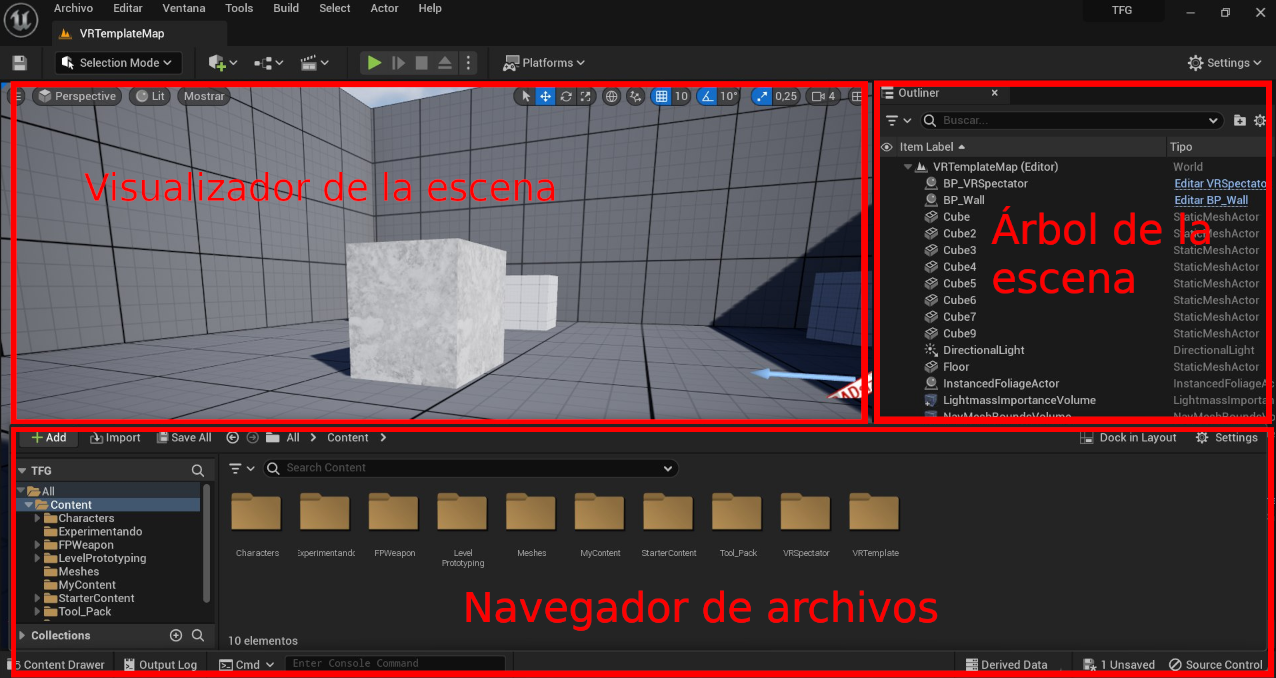
\includegraphics[width=10cm]{imagenes/unrealinicio}
	\caption{Editor de Unreal Engine 5.}
	\label{fig:unrealinicio}
\end{figure}

En el desarrollo de ChiselVR se han usado, aparte de distintos modelos 3D y efectos que se mencionarán a su debido tiempo, cuatro elementos principales: \texttt{BP\_Block} y \texttt{BP\_Debri} en la carpeta \textit{/Content/MyContent}, los cuales han sido creados desde cero, y \texttt{VRPawn} y \texttt{WidgetMenu}, elementos plantilla que han sido modificados y expandidos y que se encuentran en \textit{/Content/VRTemplate/Blueprints}.

Una vez añadido el plugin Geometry Script, se inicia la implementación.

\section{Gestión de colisiones en Unreal Engine}

Unreal Engine ofrece un sistema de colisiones y respuestas muy completo del cual ChiselVR saca provecho. Este sistema permite configurar una serie de propiedades en distintos tipos de objetos, de forma que \textbf{las interacciones entre unos tipos y otros puedan ser distintas y personalizadas}. En este proyecto se trabaja con estas propiedades, haciendo que, por ejemplo, el disco de la radial solape o bloquee dependiendo de si se enciende o no, o que el evento de choque del cincel con el martillo se dispare únicamente si este golpea la parte trasera del cincel. Otra ventaja importante de configurar las propiedades de las colisiones es \textbf{el rendimiento}. Gestionado correctamente, los diferentes objetos esperarán eventos de colisión únicamente de aquello que es necesario, por lo que conllevarán un \textbf{coste computacional considerablemente menor}.

\section{\texttt{BP\_Block}}

\begin{figure}[H]
	\centering
	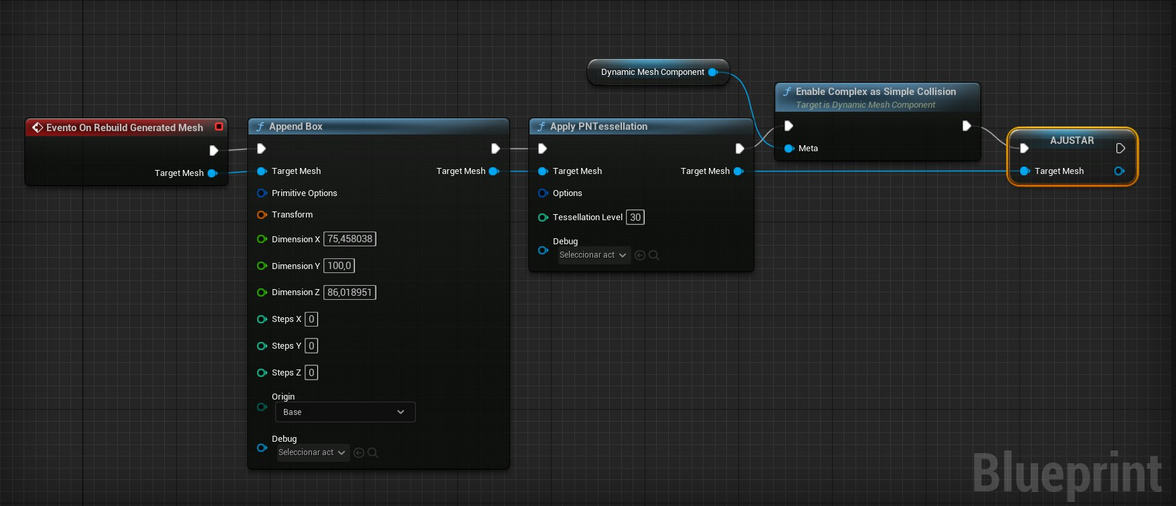
\includegraphics[width=8cm]{imagenes/bpblock}
	\caption{Blueprint de \texttt{BP\_Block}.}
	\label{fig:bpblock}
\end{figure}

\begin{figure}[H]
	\centering
	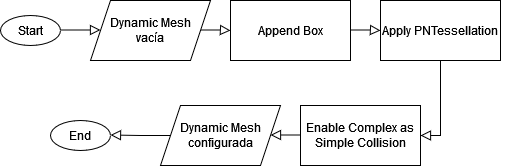
\includegraphics[width=8cm]{imagenes/flowchart1}
	\caption{Diagrama de flujo de \texttt{BP\_Block}.}
	\label{fig:fc1}
\end{figure}

El Blueprint \texttt{BP\_Block} fue el primero en implementarse, y en torno al que gira todo el proyecto. Es una clase heredada de \texttt{GeneratedDynamicMeshActor}, clase que proviene de Geometry Script y a la cual se le pueden aplicar las operaciones booleanas que necesitamos. Técnicamente, se podría usar solamente el componente \texttt{DynamicMeshComponent}, al cual también se le pueden aplicar operaciones booleanas, pero para este proyecto \textbf{es necesario usar el objeto actor} por una de sus funciones: \texttt{EventOnRebuildGeneratedMesh}. Esta función actua como un constructor en una clase convencional, pero permite, al ser posible su uso dentro de la propia Blueprint, una mayor versatilidad en la creación de la malla, además de mayor rendimiento en el editor (información extraída de la documentación oficial\footnote{\url{https://docs.unrealengine.com/5.0/en-US/geometry-script-users-guide/}}). El elemento \texttt{Target Mesh} de esta función es la malla dinámica que da forma a este actor, y sobre la que se aplican las modificaciones.

El funcionamiento de \texttt{EventOnRebuildGeneratedMesh} sigue así: primero, se le da forma con la función \texttt{AppendBox}, la cual añade una primitiva en forma de caja a la malla dinámica. Así se obtiene la forma de bloque. Una vez hecho esto, se aplica una subdivisión de triángulos usando la función \texttt{ApplyPNTessellation}. Esto es necesario para obtener un mejor rendimiento al aplicar las operaciones booleanas ya que facilita el recálculo de la topología de los triángulos. Por último, se añade colisión con la función \texttt{EnableComplexAsSimpleCollision}. Como se ha explicado previamente, normalmente las mallas de colisión son versiones simplificadas de la malla visible, pero en casos concretos se usa una malla de colisión lo más cercana posible a la visible. Unreal Engine da la posibilidad de configurar ambas, y de \textbf{usar una en lugar de la otra}. Con esta función, se usa la malla compleja en lugar de la simple, lo cual permite que, siempre que alguna herramienta colisione con el bloque, \textbf{choque siempre contra la superficie visible de este} y no contra el aire, ya que nunca se usa la versión simplificada. Una vez hecho todo esto, se aplican los cambios (\texttt{Set}) a la malla dinámica.

Originalmente, la realización de las operaciones booleanas daba lugar dentro de este Blueprint, pero un análisis posterior concluyó en que el enfoque más correcto era que se realizase dentro del código del jugador, en \texttt{VRPawn}. Por tanto, se explicará posteriormente. Destacar también que en el esquema del Blueprint se pueden apreciar líneas azules (variables) surgiendo de dos lados distintos: \texttt{Target Mesh} y \texttt{Dynamic Mesh Component}. Estas variables \textbf{son la misma}, una por referencia y la otra no, y se están usando al mismo tiempo únicamente por requerimiento de las funciones usadas, por eso no se han tenido en cuenta a la hora de diseñar el diagrama de flujo.

\section{\texttt{VRPawn}}

Este Blueprint equivale al usuario, y es donde toda su interacción con el mundo se lleva a cabo. Por tanto, es también donde se realizan todas las operaciones de las herramientas, las cuales estaban implementadas dentro de \texttt{BP\_Block} hasta cierto punto del desarrollo del martillo y cincel.

\subsection{Construcción}

\begin{figure}[H]
	\centering
	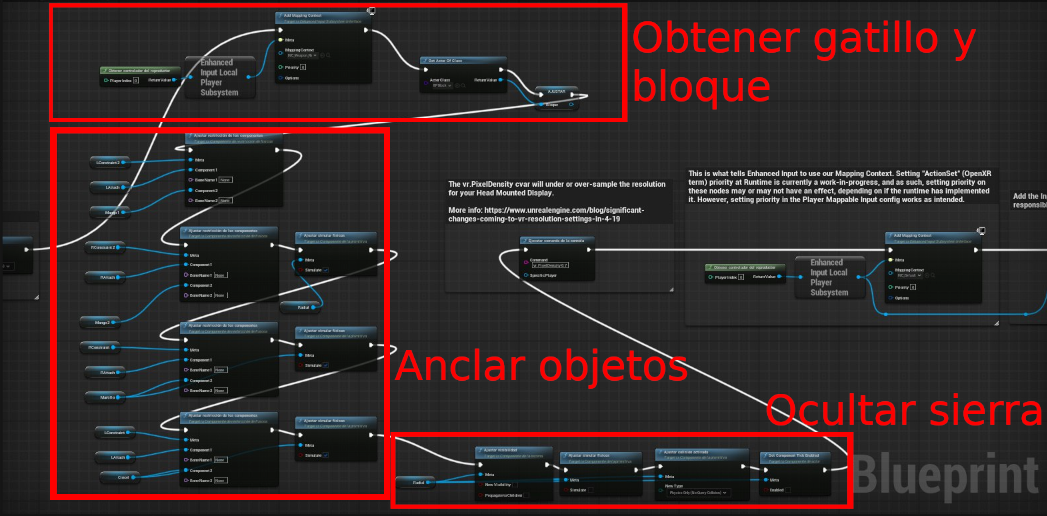
\includegraphics[width=9.2cm]{imagenes/constructor}
	\caption{\texttt{EventBeginPlay} de \texttt{VRPawn}.}
	\label{fig:constructor}
\end{figure}

\begin{figure}[H]
	\centering
	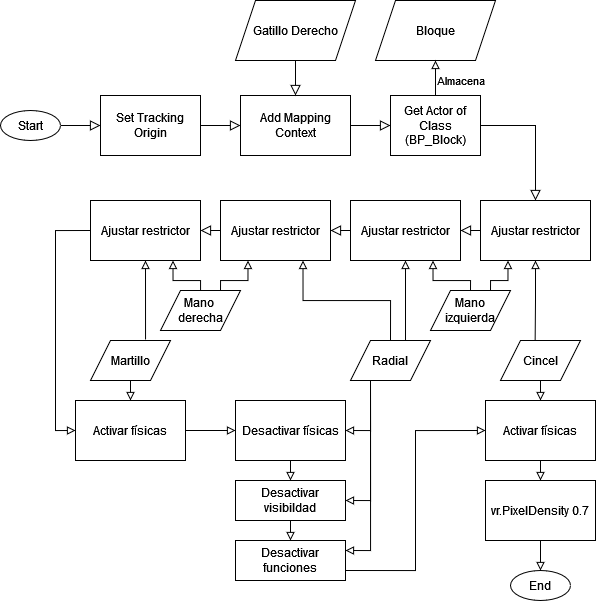
\includegraphics[width=12cm]{imagenes/flowchart2}
	\caption{Diagrama de flujo de \texttt{EventBeginPlay}.}
	\label{fig:fc2}
\end{figure}

\texttt{VRPawn} cuenta por defecto con una función llamada \texttt{EventBeginPlay}, la cual sirve para ejecutar una serie de elementos al iniciar la aplicación (como podrían ser el seguimiento de la posición del usuario o el mapeado de los controles). Por tanto, con cada nueva funcionalidad, es aquí donde deberán añadirse las partes de dicha funcionalidad que deban ejecutarse con el inicio de la aplicación.

Comentar que en este punto es también donde la plantilla modifica la variable \texttt{vr.PixelDensity}, la cual sirve para cambiar la resolución nativa de la aplicación. Para mejorar el rendimiento de la aplicación, se ha establecido dicha variable en 0.7, es decir un 70\% del valor predeterminado.

Los elementos tratados en esta función son los siguientes:

\begin{itemize}
    \item Obtener reconocimiento del gatillo derecho con \texttt{AddMappingContext} para su uso en la sierra radial.
    \item Obtener el objeto Bloque de la escena para almacenarlo como variable usando \texttt{GetActorOfClass}. Esto pasó a ser necesario al cambiar el código de las herramientas de \texttt{BP\_Block} a \texttt{VRPawn}, cambio que se hizo para un mejor manejo de las coordenadas y del cambio entre coordenadas globales y locales.
    \item Anclar todas las herramientas a los restrictores físicos. Para conseguir que las herramientas pudiesen colisionar con objetos y seguir el movimiento de las manos al mismo tiempo, se usaron \textbf{restrictores físicos}, los cuales unen dos objetos y permiten configurar diferentes parámetros sobre esta unión. De esta forma, las herramientas \textbf{siempre están en una posición natural respecto a las manos, excepto cuando un obstáculo las bloquea}. En esta función es cuando se indica qué componentes están anclados entre sí.
    \item Ocultar la sierra radial, ya que la herramienta inicial es el martillo y cincel. Para hacer esto, se desactiva su visibilidad, su colisión y sus funciones.
\end{itemize}

De esta sección cabe destacar \textbf{las dificultades enfrentadas a la hora de desarrollar las manos físicas}. Durante la investigación de cómo solucionar este problema, uno de los métodos probados fue usando la función \texttt{SetTarget LocationAndRotation}, de forma que las manos simuladas estuviesen continuamente teletransportandose a la posición de las manos reales. Esta solución, aunque útil en algunos casos, no lo es para ChiselVR, ya que únicamente sirve para dar la ilusión de choque al aplicar una fuerza leve, pero con suficiente insistencia acaba atravesando superficies sólidas. Al seguir investigando se llegó a la solución actual, en la que en lugar de teletransportarse, las manos simuladas \textbf{siguen} a las reales, chocando por el camino.

\subsection{Cincel y martillo}

\begin{figure}[H]
	\centering
	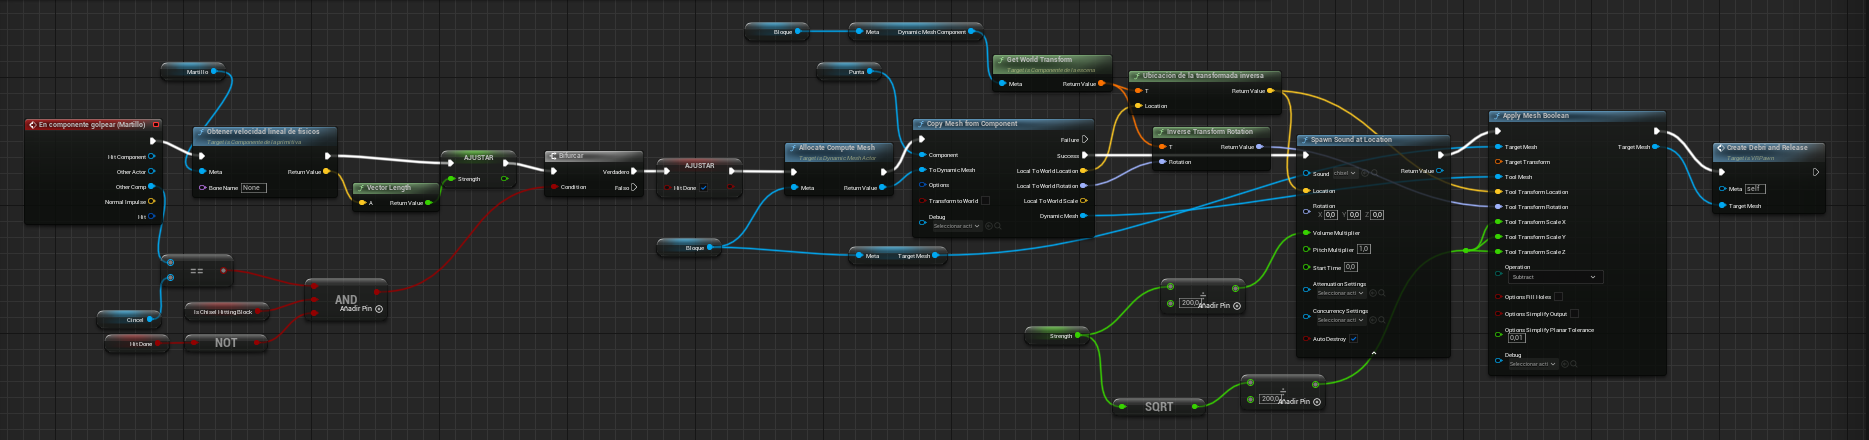
\includegraphics[width=12cm]{imagenes/martilloycincel}
	\caption{Función para cincel y martillo de \texttt{VRPawn}.}
	\label{fig:martilloycincel}
\end{figure}

\begin{figure}[H]
	\centering
	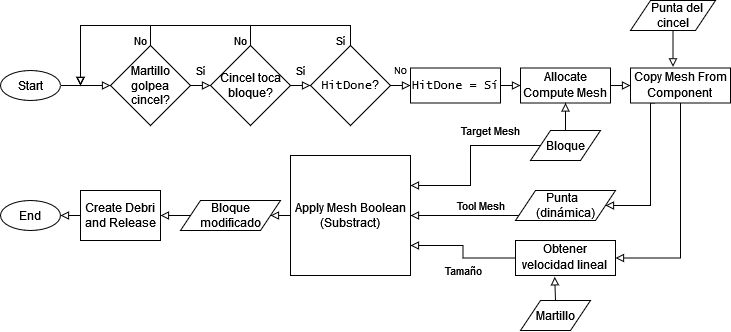
\includegraphics[width=12cm]{imagenes/flowchart3}
	\caption{Diagrama de flujo del cincel y martillo.}
	\label{fig:fc3}
\end{figure}

Esta herramienta ha sido probablemente el elemento de ChiselVR que más cambios ha tenido. Desde retoques en las colisiones a ajustes en la forma de realiza la operación booleana, el código del cincel y martillo ha pasado por diversas iteraciones para llegar a un punto en el que funcione como se esperaría. Ahora repasaremos su evolución y funcionamiento.

El primer problema a tener en cuenta es \textbf{qué se considera un golpe}. En las primeras iteraciones, un error en el funcionamiento surgía: al dar un golpe, se realizaba más de una operación. Este problema se origina en la detección de colisiones, ya que por cada \textit{tick} de la aplicación en el que tanto el bloque como el martillo estuviesen tocando el cincel, la operación se aplicaba. El movimiento humano no es lo suficientemente rápido como para realizar el golpe en un único \textit{tick}, por lo que la operación podía realizarse múltiples veces en un único golpe.

Para solucionar este problema, se crearon dos variables booleanas, \texttt{HitDone} e \texttt{IsChiselHittingBlock}, acompañadas de dos cajas de colisión en la cabeza del martillo y la punta del cincel, respectivamente. La segunda es más sencilla, simplemente cambia entre verdadero y falso dependiendo de si la caja de colisión de la punta del cincel se superpone con el bloque. La primera es algo más compleja: la variable \texttt{HitDone} empieza en falso. Cuando el martillo golpea al cincel, esta se cambia a verdadero, lo cual evita que la operación se vuelva a ejecutar de seguido con una bifurcación. Para que vuelva a estar en falso y, por tanto, se pueda realizar una nueva operación, \textbf{el cincel debe abandonar el área que compone la caja de colisiones que cubre la cabeza del martillo}. De esta forma, es necesario apartar ligeramente el martillo del cincel para volver a realizar una operación booleana, imitando así la necesidad de reunir algo de fuerza para el impacto al esculpir en la vida real (Figura \ref{fig:hitdone}).

\begin{figure}[H]
	\centering
	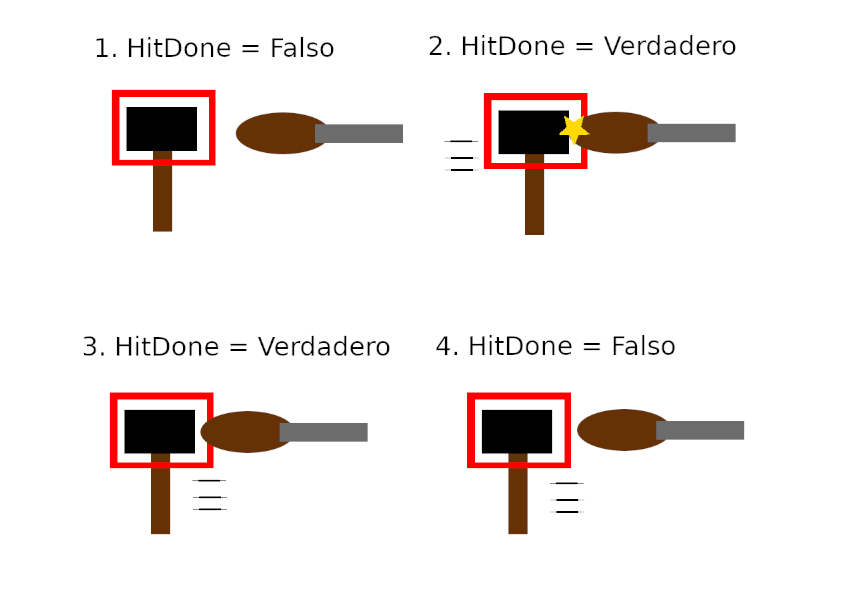
\includegraphics[width=7cm]{imagenes/hitdone}
	\caption{Esquema de la detección del golpe.}
	\label{fig:hitdone}
\end{figure}

Con este sistema, el problema de saber cuándo realizar una operación y cuándo no está solucionado. Con esto, el cálculo de la operación es más directo. Primero, se aloja una malla dinámica temporal copiando la malla de la punta del cincel, ya que las operaciones booleanas solo se pueden realizar entre mallas dinámicas. Una vez alojada, se obtiene la localización donde se realizará la operación. \textbf{La función \texttt{ApplyMeshBoolean} requiere que se le de la posición y la rotación de la herramienta en las coordenadas locales del bloque}, por lo que obtenemos las coordenadas globales de la herramienta y del bloque, y al usar la inversa de la transformación del bloque sobre la herramienta, conseguimos traducir la ubicación de esta a las coordenadas locales del bloque (Figura \ref{fig:transformacion}). Esta traducción fue costosa de alcanzar (fue una de las principales razones por la que se trasladó el código de \texttt{BP\_Block} a \texttt{VRPawn}) ya que consiste en un doble recálculo de la matriz de transformación de un objeto, lo cual requiere de \textbf{visión espacial y lógica} para realizarse correctamente, sobretodo en 3D. Con la ubicación del golpe obtenida, se aplica la operación con el tamaño dependiendo de la velocidad con la que se usase el martillo, se crean los restos si quedan trozos flotantes (se explicará el funcionamiento de esto más adelante) y se liberan todas las mallas temporales para evitar fugas de memoria.

\begin{figure}[H]
	\centering
	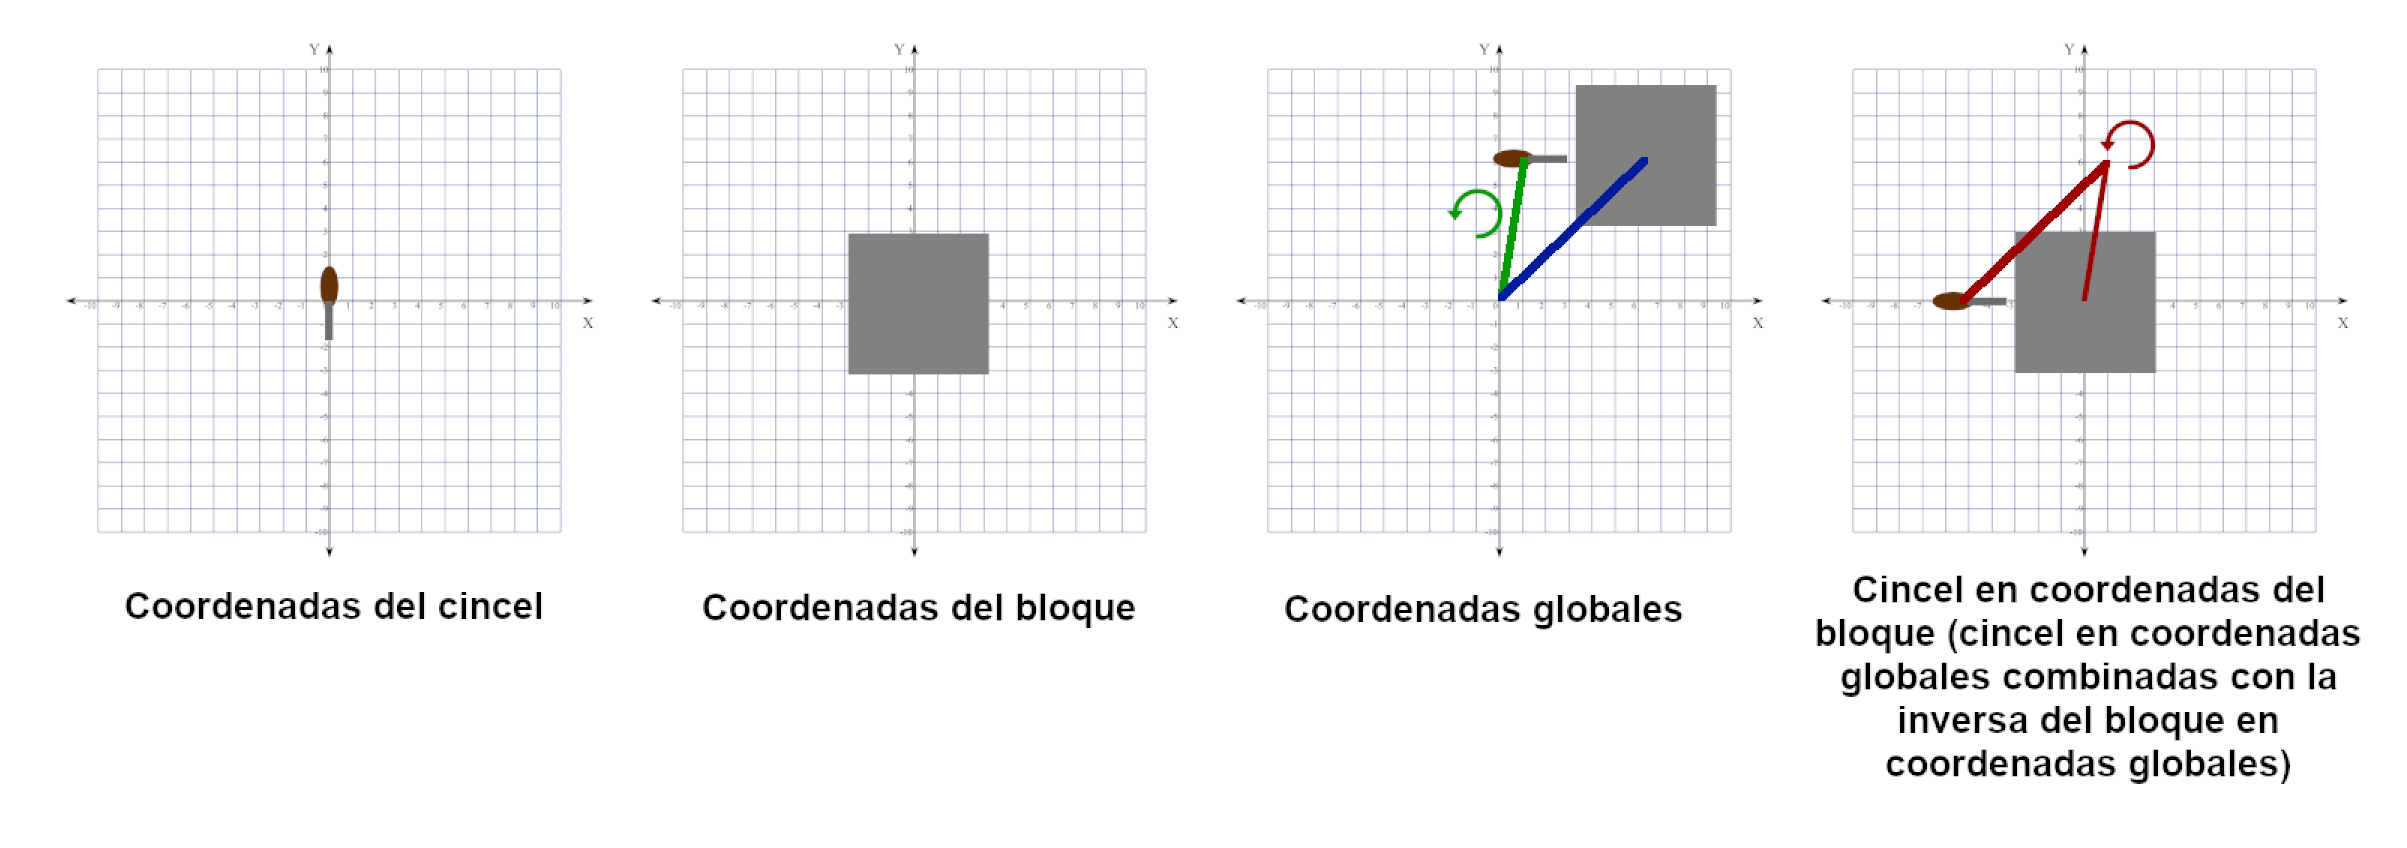
\includegraphics[width=12.5cm]{imagenes/transformacion}
	\caption{Transformación para realizar la operación booleana.}
	\label{fig:transformacion}
\end{figure}

\subsection{Sierra radial}

\begin{figure}[H]
	\centering
	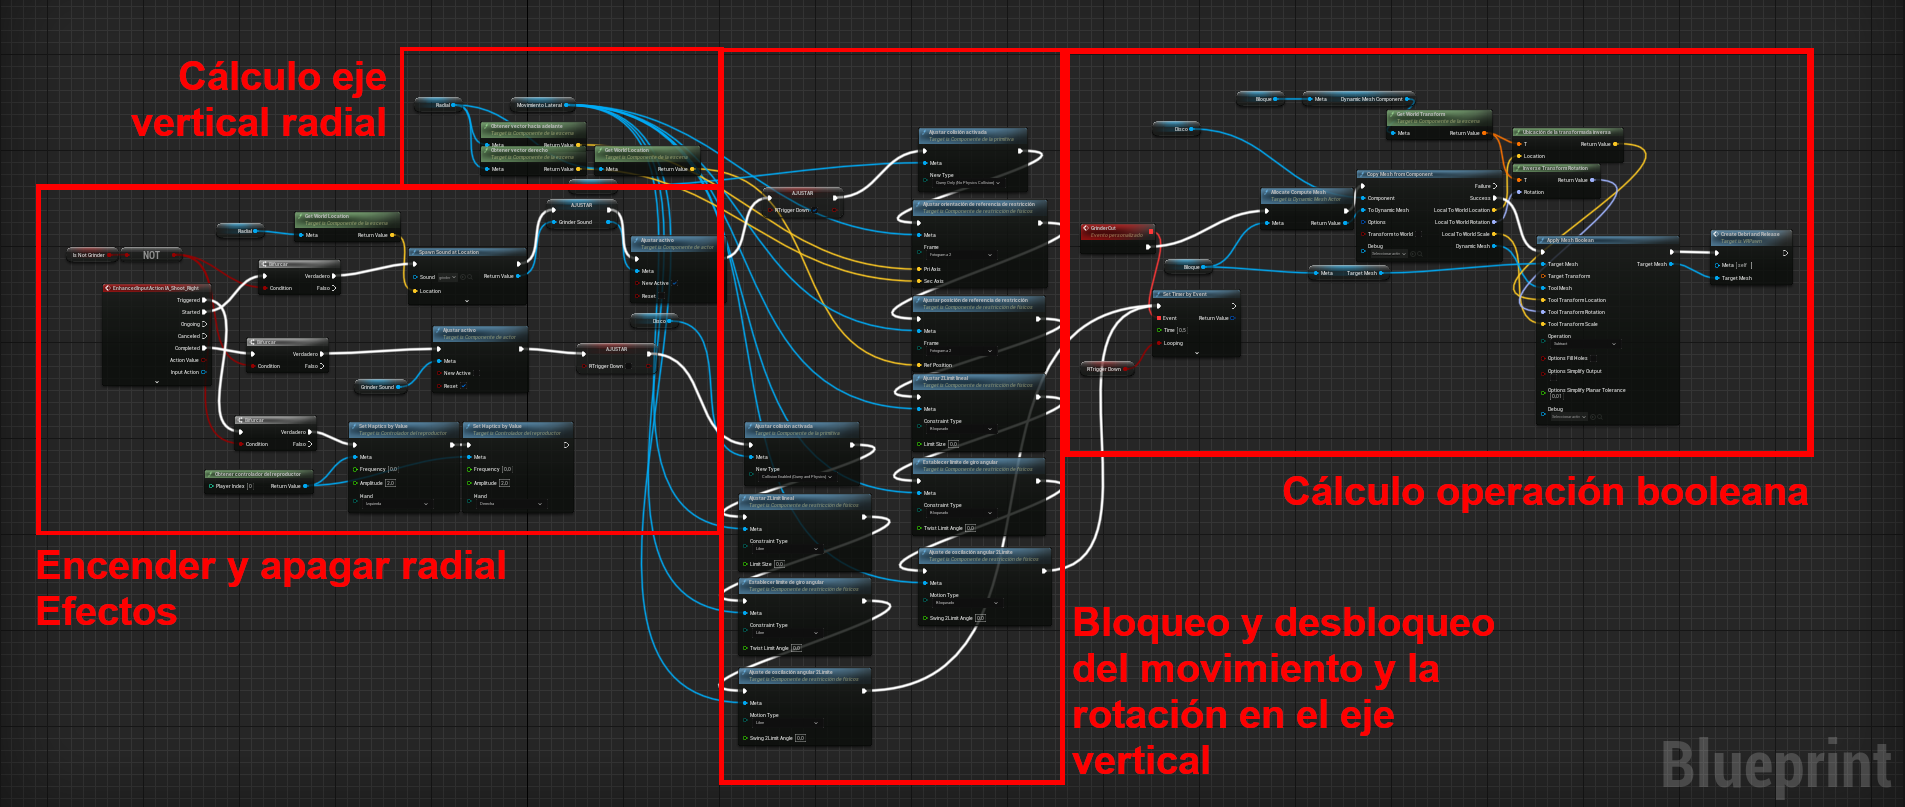
\includegraphics[width=12.5cm]{imagenes/radial}
	\caption{Función para la radial de \texttt{VRPawn}.}
	\label{fig:radial}
\end{figure}

\begin{figure}[H]
	\centering
	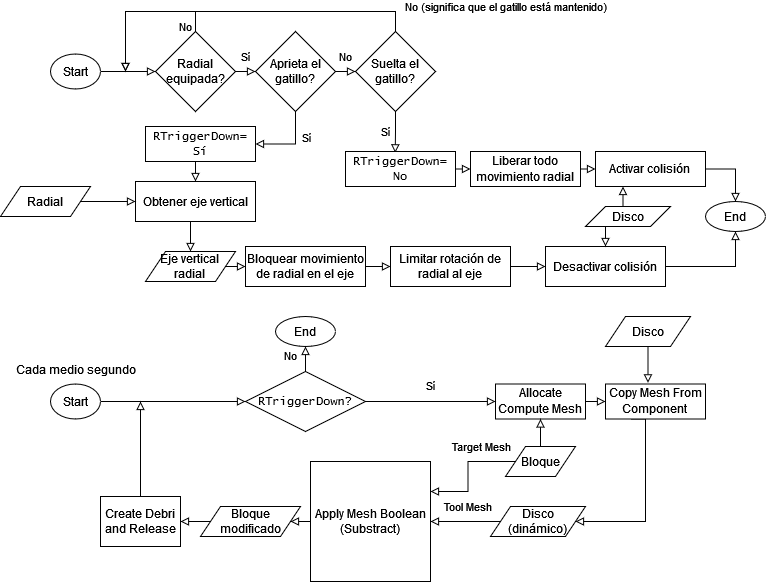
\includegraphics[width=12.2cm]{imagenes/flowchart4}
	\caption{Diagrama de flujo de la radial.}
	\label{fig:fc4}
\end{figure}

Esta herramienta hereda parte del funcionamiento del martillo y cincel, principalmente la propia realización de la operación booleana, la localización de esta y la creación de restos. Más allá de eso, tiene un funcionamiento muy distinto. En primer lugar, esta herramienta \textbf{se coge con ambas manos}, por lo que fue necesario usar prueba y error para ajustar los puntos de anclaje de las manos para que la sensación de estar sosteniendo la herramienta fuese correcta y realista. Este fue el punto más sencillo de solucionar, los siguientes provocaron más complicaciones.

Para activar la herramienta, es necesario pulsar el gatillo del mando derecho, imitando así la realidad. Con la función \texttt{EnchancedInputActionIA\_Shoot\_Right}, podemos controlar de forma precisa qué hacer dependiendo de cómo se pulse: al empezar a pulsar, cuando está mantenido, cuando se suelta, etc. Para la función de cortar material, se han usado los disparadores de \textbf{al pulsar y al soltar}. Primero, en ambos casos, se comprueba que la herramienta en uso es la sierra. Una vez comprobado, en caso de empezar a pulsar, se desactiva la colisión del disco de la sierra para que este pueda atravesar, se fija el movimiento de la herramienta a un plano paralelo a dicho disco y se activa la realización de la operación booleana con una repetición cada medio segundo. Al soltar el gatillo, se desactivan las restricciones de movimiento y la función de las operaciones, y se rehabilita la colisión del disco (Figura \ref{fig:grinder_collision}).

\begin{figure}[H]
	\centering
	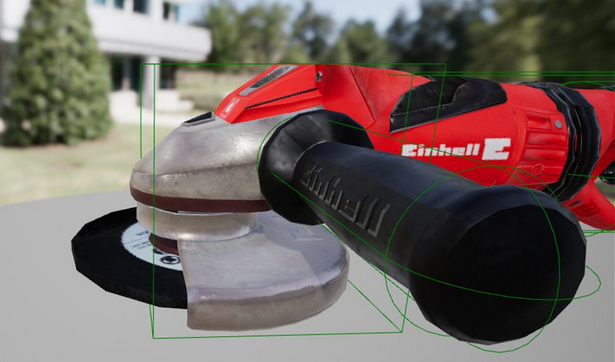
\includegraphics[width=6.3cm]{imagenes/grinder_collision}
	\caption{Malla de colisión creada para la sierra radial. La colisión del disco va aparte para que pueda chocar o no dependiendo de si está en movimiento.}
	\label{fig:grinder_collision}
\end{figure}

El factor más costoso de desarrollar para esta herramienta fue \textbf{limitar el movimiento de la sierra mientras esta está encendida}. La razón para esta limitación es evitar situaciones surrealistas al cortar el bloque: la parte que corta del disco es el borde, no la superficie, por lo que si la sierra se moviese de forma libre en todas direcciones mientras se corta no tendría sentido. Es necesario bloquear el movimiento vertical para que el corte resultante sea creíble.

Con este objetivo en mente, se abarcó el problema de distintas formas, la mayoría sin éxito. \textbf{Las formas que facilita Unreal Engine para bloquear el movimiento únicamente funcionan respecto a ejes de la escena}, por lo que el bloqueo funcionaba para mover la herramienta de forma paralela al suelo. Este obviamente no era el funcionamiento deseado, por lo que se tuvo que buscar otra forma. Finalmente, se encontraron una serie de funciones que permiten bloquear el movimiento de un objeto a partir de un plano dado, el cual se tiene que dar usando los vectores hacia delante y hacia la derecha de dicho plano. Obteniendo estos vectores de la radial y usándolos como parámetros en dichas funciones, se consiguió bloquear el movimiento en el plano deseado. Se puede ver cómo se llama a estas funciones en la parte central de la figura \ref{fig:radial}.

\subsection{Caída de escombros flotantes}

\begin{figure}[H]
	\centering
	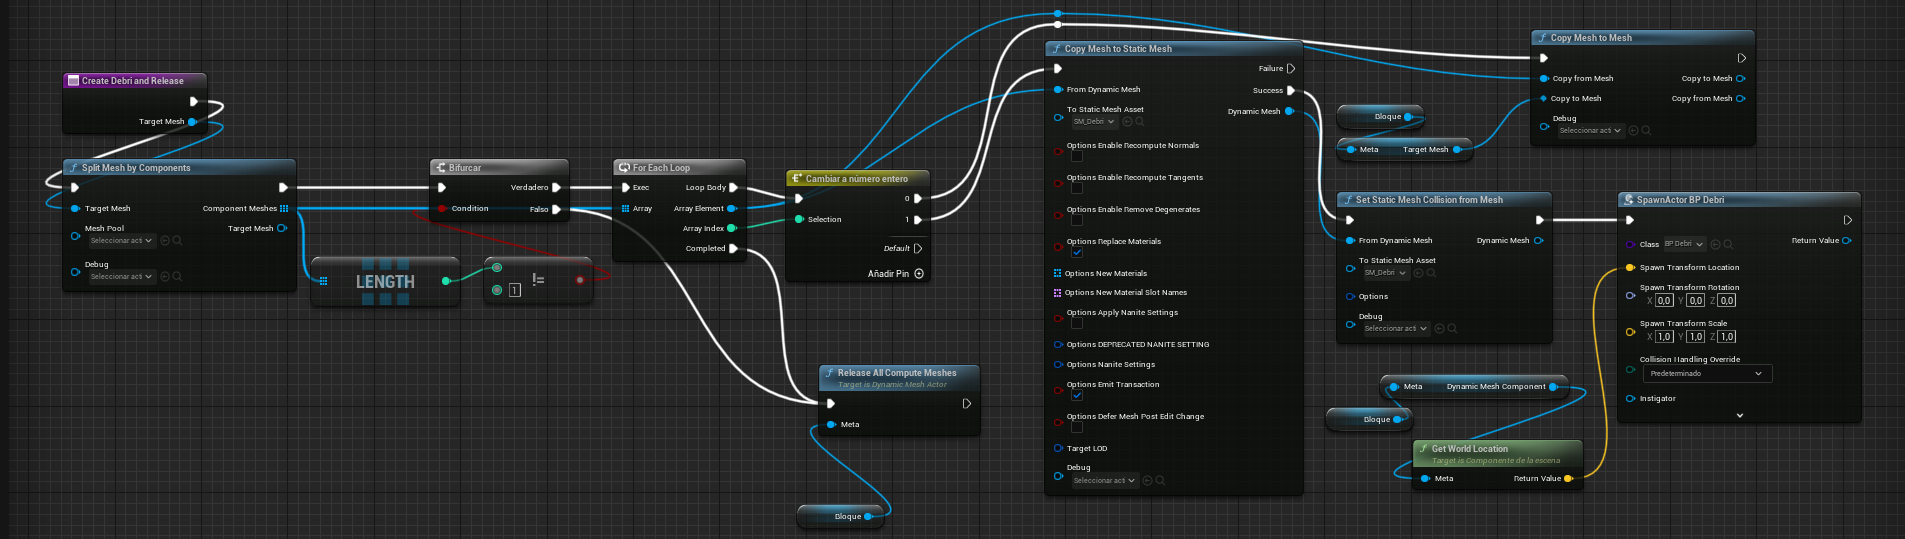
\includegraphics[width=12cm]{imagenes/createdebri}
	\caption{Función \texttt{CreateDebriAndRelease} de \texttt{VRPawn}.}
	\label{fig:createdebri}
\end{figure}

\begin{figure}[H]
	\centering
	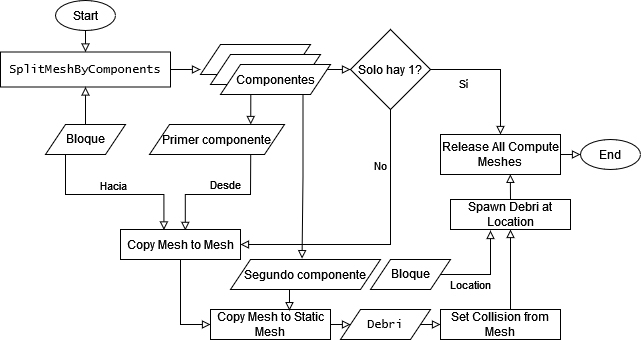
\includegraphics[width=12cm]{imagenes/flowchart5}
	\caption{Diagrama de flujo de \texttt{CreateDebriAndRelease}.}
	\label{fig:fc5}
\end{figure}

El elemento más importante a tener en cuenta respecto a efectos inmersivos fue la caída de escombros flotantes. Esto consiste en que, al realizar una operación booleana, \textbf{pueden quedar trozos inconexos del bloque principal}. Normalmente, estos trozos quedarían flotando, por lo que fue necesario implementar una forma de que cayeran al suelo.

Tras una larga investigación para ver si esto era siquiera posible, se encontró una función que nos facilita Geometry Script: \texttt{SplitMeshByComponents}. Esta función recibe una malla dinámica, detecta a través de los datos geométricos de esta todos los componentes independientes que la forman y devuelve una lista con todos estos componentes. En la documentación no se especifica cuál es el orden por defecto en el que se ordena esta lista, pero posterior experimentación concluye que es por \textbf{la altura del punto más bajo de cada componente}, siendo el primero el más bajo. Este orden nos viene perfecto, pues esto significa que el primer puesto de la lista siempre será la parte del bloque que aún está tocando el suelo y, por tanto, la que queremos que se quede.

Una vez accesibles los trozos en los que se divide el bloque, simplemente se itera sobre la lista dada: el primer objeto sustituirá al anterior bloque, de forma que este pasará a ser el mismo que antes pero sin los trozos flotantes. El siguiente trozo se guardará en un asset variable, \texttt{SM\_Debri}, el cual es el único componente del Blueprint \texttt{BP\_Debri}. Una vez guardado, se invoca un actor de la clase \texttt{BP\_Debri} en las mismas cordenadas que el propio bloque, de forma que el trozo de malla dinámica flotante es sustituido por una instancia de \texttt{BP\_Debri}, la cual tiene una cuenta atrás de autodestrucción de 5 segundos para ahorrar recursos. Una vez invocada, se le aplican colisiones simples y físicas, de forma que \textbf{cae al suelo de forma realista} (Figura \ref{fig:debri}).

\begin{figure}[H]
	\centering
	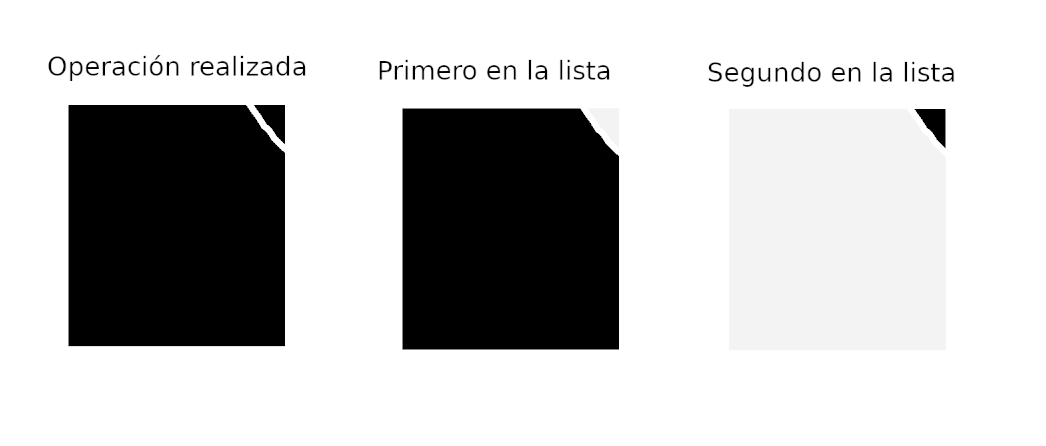
\includegraphics[width=8cm]{imagenes/debri}
	\caption{Resultado de la separación por componentes. Tanto el bloque original como los resultantes comparten exactamente las mismas coordenadas.}
	\label{fig:debri}
\end{figure}

Se podría dar la ocasión de que hubiesen más de un escombro resultante de una operación, pero por la rareza de este caso y lo pesado que podría ser computacionalmente, se ha ignorado.

Una vez hecho todo esto, se acaba la iteración por la lista. Esta función, junto a la liberación de mallas temporales para evitar fugas de memoria, están recogidos dentro de la función \texttt{CreateDebriAndRelease}, la cual se creó ya que todas las herramientas comparten este funcionamiento al final de sus respectivos códigos.

\subsection{Efectos de sonido y hápticos}

Añadir que en \texttt{VRPawn} es también donde se incluyen los diferentes efectos añadidos para la inmersión. En el caso del \textbf{martillo y cincel}, se reproduce una vibración y un sonido al mismo tiempo que se realiza la operación booleana, los cuales también varían dependiendo de la \textbf{velocidad del martillo}. En el caso de la \textbf{sierra radial}, un efecto de sonido empieza \textbf{al presionar el gatillo}, y se lanza una petición al mezclador de sonido para pararlo y reiniciarlo cuando el gatillo se suelta. Para la vibración, se mantiene una vibración constante todo el tiempo que se mantenga el gatillo pulsado.

\section{\texttt{WidgetMenu}}

Otro de los blueprints ya implementado por la plantilla es \texttt{WidgetMenu}, el cual ofrece una base para construir tu propio menú de opciones. ChiselVR contiene un total de cinco opciones las cuales funcionan así:

\begin{itemize}
    \item \textbf{Reiniciar}. Se llama a la función \texttt{OpenLevel} y se carga la misma escena.
    \item \textbf{Salir}. Se llama a la función \texttt{QuitGame}.
    \item \textbf{Cambiar mano}. Con la función \texttt{GetActorOfClass(VRPawn)} se obtiene al usuario, se comprueba el estado de la variable \texttt{HandsChanged} y, dependiendo de su estado, se ajusta para que cada mano obtenga sus datos de movimiento de un mando distinto. Al principio, se intentó cambiar físicamente la herramienta de una mano a otra, pero de esta otra forma se simplifica el código y se mantiene dentro de \texttt{WidgetMenu}. Esta función está desactivada cuando se tiene la sierra radial en las manos, pues esta solo tiene una forma de uso (Figuras \ref{fig:changedominant} y \ref{fig:fc6}).
    \item \textbf{Cincel y Martillo}. Con la función \texttt{GetActorOfClass(VRPawn)} se obtiene al usuario y se reactivan la visibilidad, físicas, colisiones y funciones de su martillo y cincel, a la vez que se teletransportan a sus manos. También se desactivan estos campos de la sierra radial, se indica con una variable booleana que la sierra radial no está activada y, en caso de que la variable \texttt{HandsChanged} esté en verdadero, se invierten las manos. Esto se debe a que, al equipar la sierra radial, las manos se ajustan a su estado original de forma automática (Figuras \ref{fig:cambiaracincel} y \ref{fig:fc7}).
    \item \textbf{Radial}. Con la función \texttt{GetActorOfClass(VRPawn)} se obtiene al usuario y se reactivan la visibilidad, físicas, colisiones y funciones de su sierra radial, a la vez que se teletransporta a sus manos. También se desactivan estos campos del martillo y cincel, se indica con una variable booleana que la sierra radial está activada y se ajustan las manos a su estado original, sea cual sea el estado de la variable \texttt{HandsChanged} (Figuras \ref{fig:cambiararadial} y \ref{fig:fc8}).
\end{itemize}

\begin{figure}[H]
	\centering
	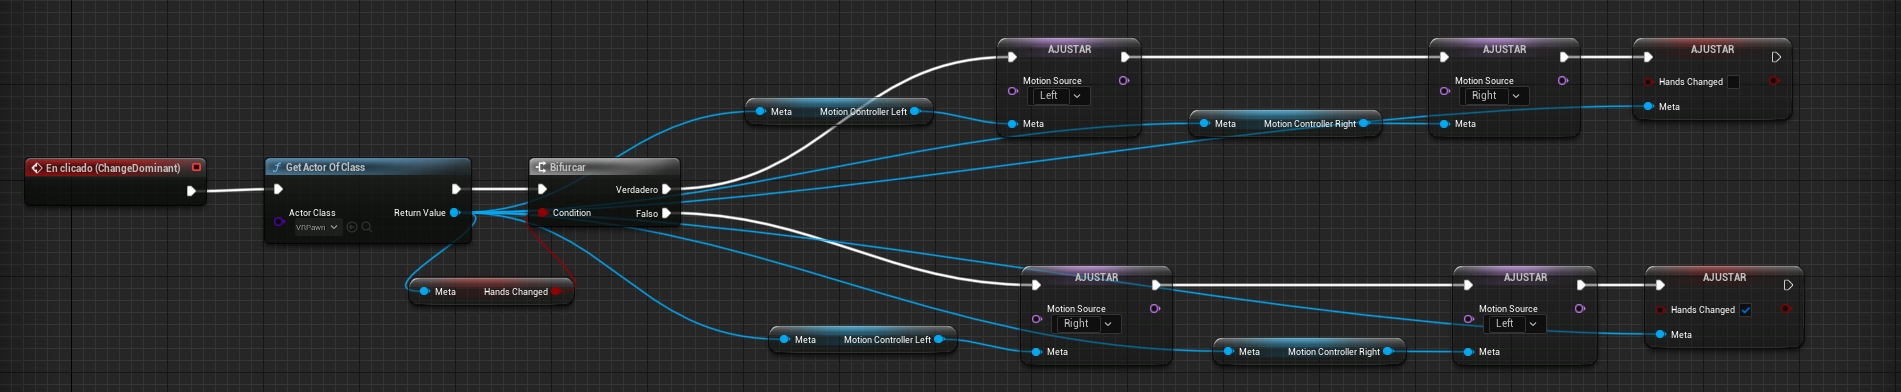
\includegraphics[width=12cm]{imagenes/changedominant}
	\caption{Función de cambio de mano en \texttt{WidgetMenu}.}
	\label{fig:changedominant}
\end{figure}

\begin{figure}[H]
	\centering
	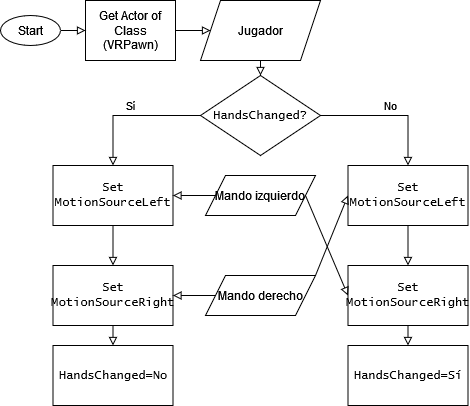
\includegraphics[width=12cm]{imagenes/flowchart6}
	\caption{Diagrama de flujo de la función de cambio de mano.}
	\label{fig:fc6}
\end{figure}

\begin{figure}[H]
	\centering
	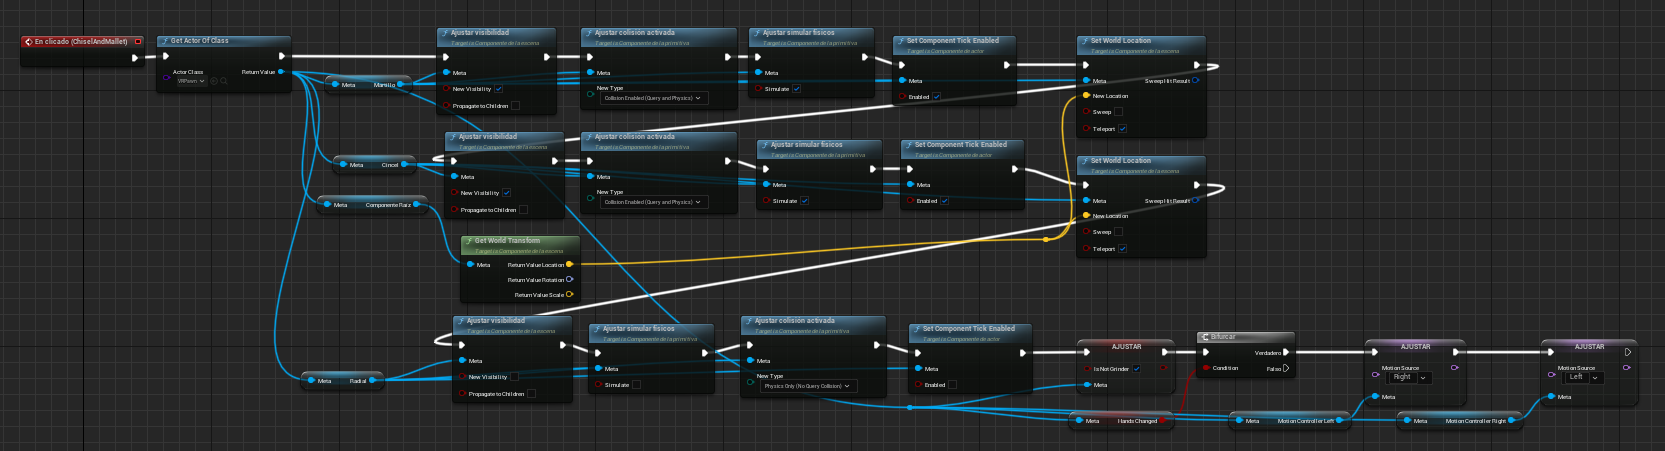
\includegraphics[width=12cm]{imagenes/cambiaracincel}
	\caption{Función de cambio a cincel y martillo en \texttt{WidgetMenu}.}
	\label{fig:cambiaracincel}
\end{figure}

\begin{figure}[H]
	\centering
	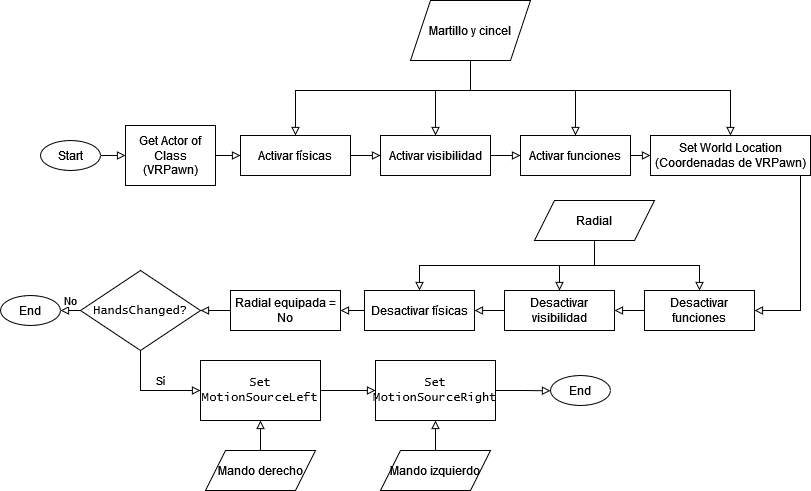
\includegraphics[width=12cm]{imagenes/flowchart7}
	\caption{Diagrama de flujo de la función de cambio a cincel y martillo.}
	\label{fig:fc7}
\end{figure}

\begin{figure}[H]
	\centering
	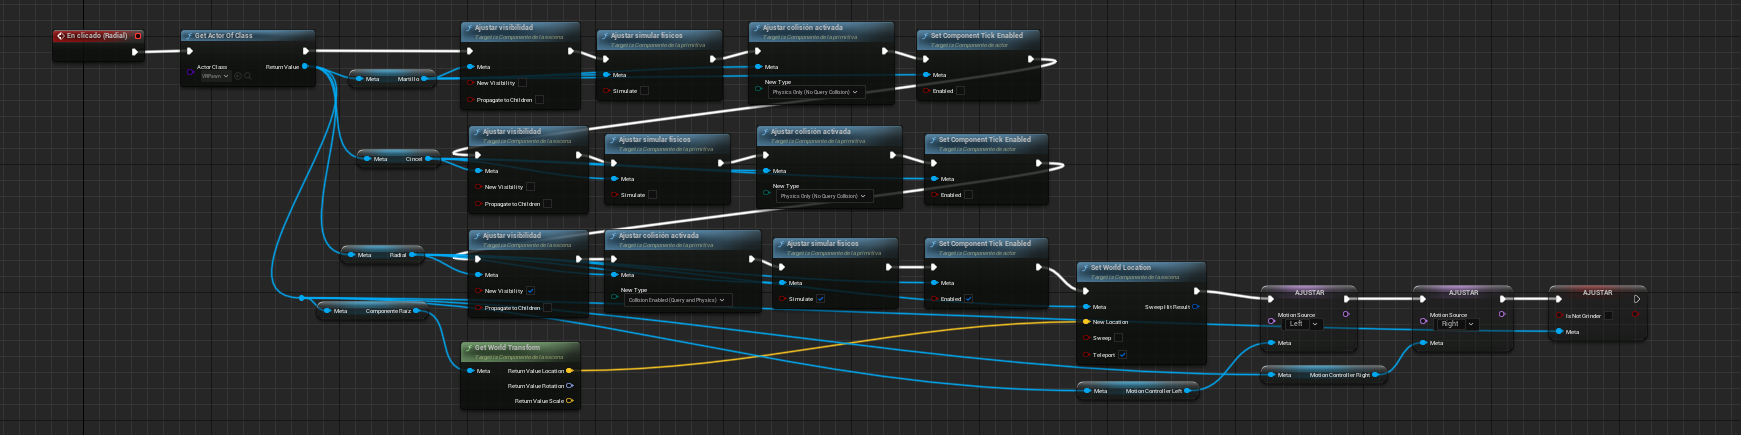
\includegraphics[width=12cm]{imagenes/cambiararadial}
	\caption{Función de cambio a radial en \texttt{WidgetMenu}.}
	\label{fig:cambiararadial}
\end{figure}

\begin{figure}[H]
	\centering
	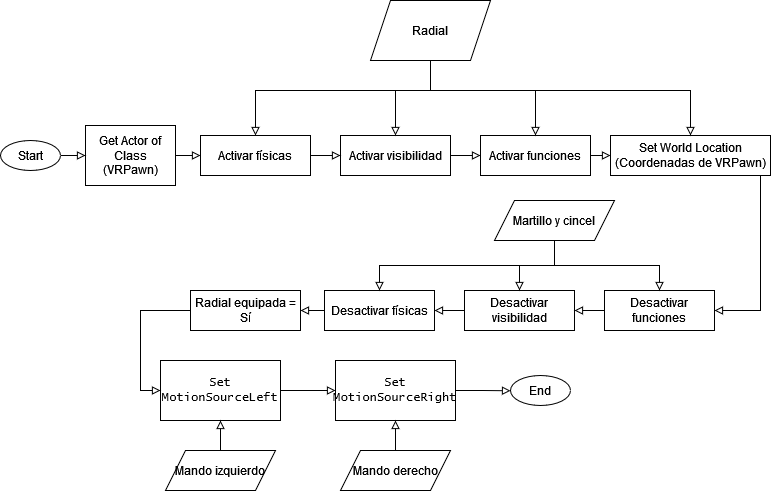
\includegraphics[width=12cm]{imagenes/flowchart8}
	\caption{Diagrama de flujo de la función de cambio a radial.}
	\label{fig:fc8}
\end{figure}

\begin{figure}[H]
	\centering
	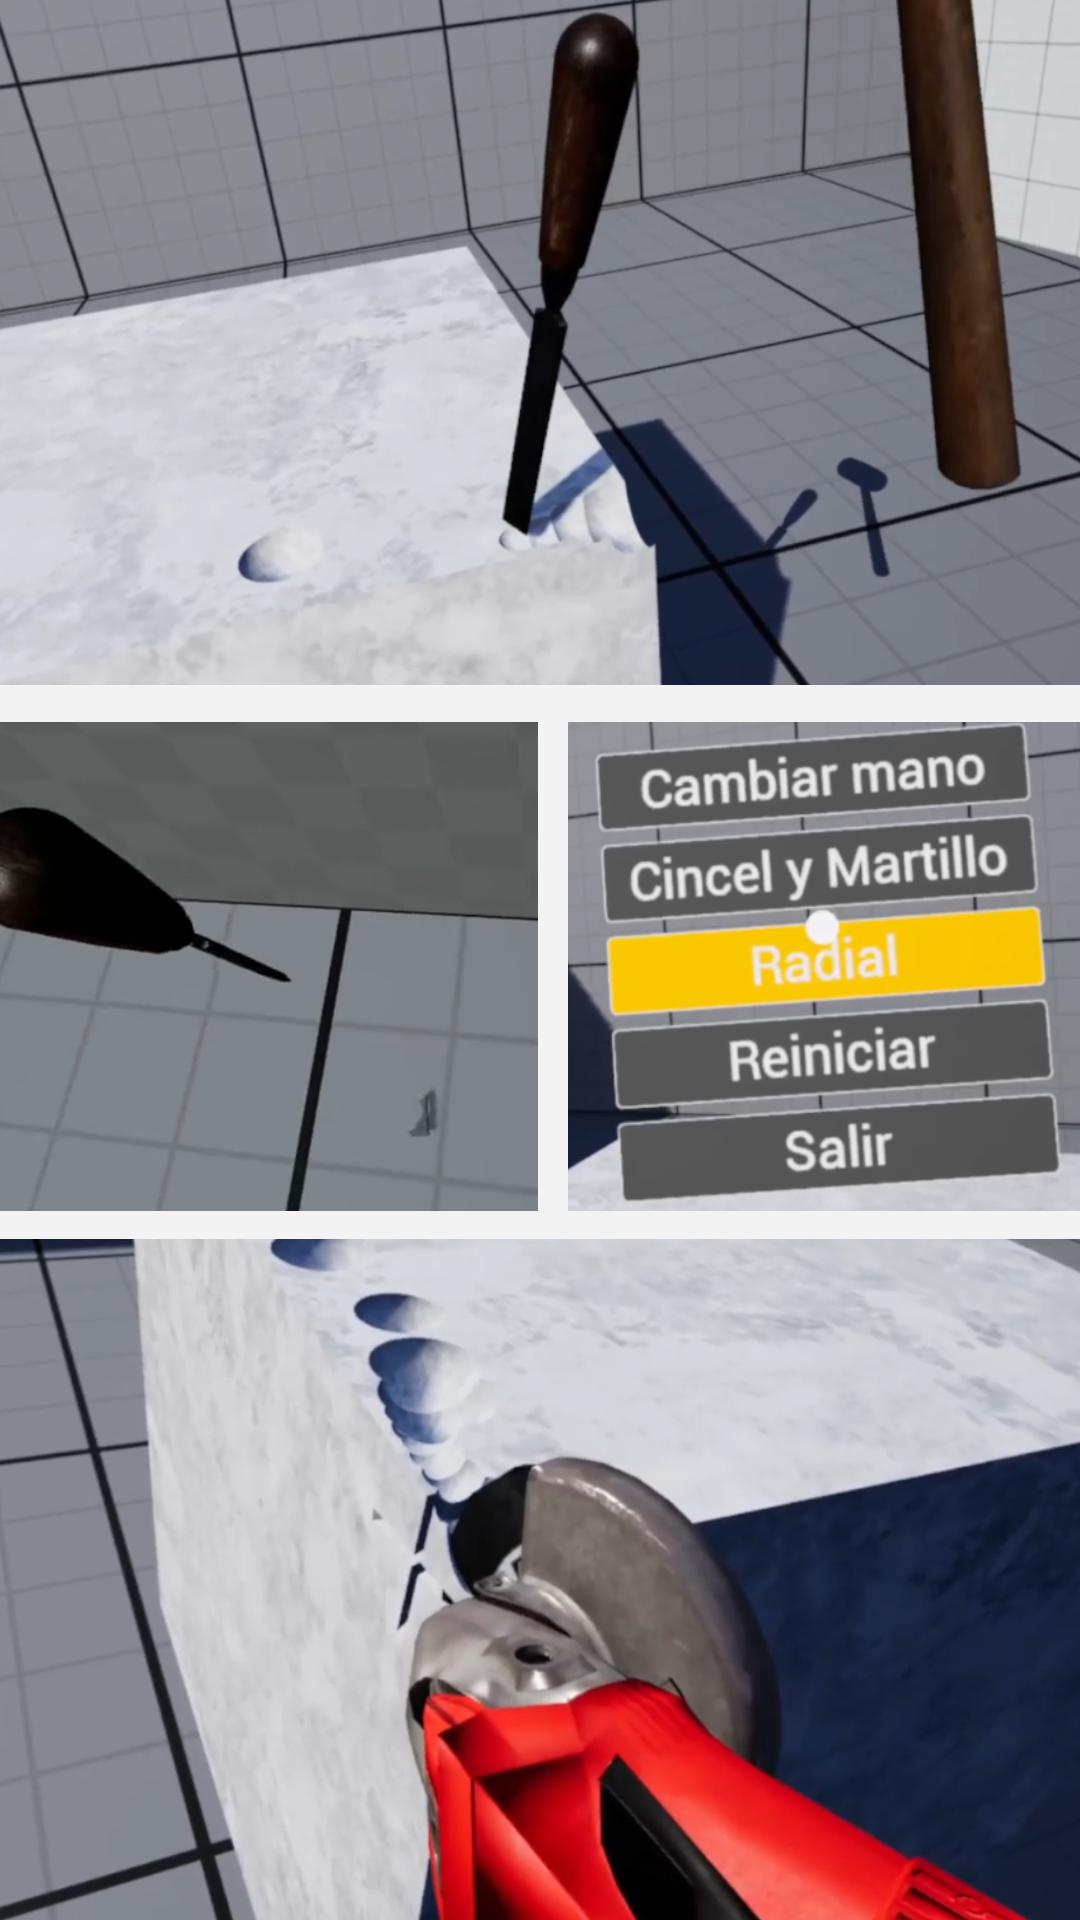
\includegraphics[width=11cm]{imagenes/screenshots}
	\caption{Capturas de pantalla de ChiselVR en ejecución.}
	\label{fig:screenshots}
\end{figure}

	\chapter{Conclusiones y trabajos futuros}

En este capítulo se verá la respuesta de los usuarios y el coste estimado del proyecto, además de conclusiones y lecciones aprendidas al acabar el desarrollo y posibles trabajos futuros respecto al proyecto o con relación a este.

\section{Encuesta a usuarios}

Se ha realizado una pequeña encuesta\footnote{\url{https://docs.google.com/spreadsheets/d/1BGSYs5X8j8LkONdlrikgJ4Nl_MxtnB71MyePUcngQuI/edit?usp=sharing}} a 8 personas con una amplia variedad de familiarización con la informática y la realidad virtual, en la cual se les ha pedido su opinión (en un valor numérico del 0 al 10) respecto a distintos aspectos de la aplicación, además de darles la oportunidad de añadir un comentario sobre sus conclusiones. Este ha sido el resultado:

\begin{itemize}
    \item Interés en la escultura en RV: \textbf{7'75}
    \item Aplicación enfocada en el realismo (0) o en el entretenimiento (10): \textbf{7'5}
    \item Interés en el realismo (0) o en el entretenimiento (10): \textbf{7'375}
    \item Interés en posterior desarrollo de la aplicación: \textbf{7'625}
    \item Interés en mejoras técnicas (0) o de contenido (10): \textbf{5'25}
\end{itemize}

En general, las opiniones son bastante directas: \textbf{la escultura en realidad virtual}, aunque no sea una idea rompedora, tiene un \textbf{interés notable}, en concreto si se enfoca más como un videojuego con mecánicas más enfocadas en el entretenimiento del usuario que en la imitación de la realidad. Respecto a la aplicación en sí, los encuestados opinan que ChiselVR se decanta más por el entretenimiento, algunos de ellos usando adjetivos como \textit{arcade} para describirla de forma positiva. También existe un \textbf{interés en el crecimiento de la aplicación en miras al futuro, aunque sin decantarse por ningún tipo en concreto}: tan llamativas son las mejoras a la estabilidad de la aplicación como lo sería añadir más opciones al usuario. Uno de los encuestados, ingeniero informático graduado, llegó a mencionar sobre esto que, aunque se notan las costuras por culpa de Geometry Script, el usuario medio no lo va a notar tanto, así que sea del tipo que sea una posible actualización sería bienvenida.

Notablemente existe una falta de encuestados provenientes del campo del arte, y por tanto, relacionados con la escultura, pero lamentablemente no se ha podido encuestar a ninguno a tiempo.

\section{Coste del proyecto}

Por un lado, estaría el salario. Se han requerido 93,5 horas reales de desarrollo, a las cuales se suman unas 10 horas de aprendizaje de las herramientas y tecnologías usadas y otros elementos varios, alcanzando las \textbf{103,5 horas}. El sueldo medio de un ingeniero de software en España es de 23.700€ al año\footnote{\url{https://www.glassdoor.es/Sueldos/ingeniero-de-software-junior-sueldo-SRCH_KO0,28.htm}}, lo cual equivale a 1.975€ al mes (si ignoramos pagas extra en el cálculo) y 12'34€ la hora. Dicho sueldo a lo largo de 103,5 horas equivale a \textbf{1.277'19€}.

Por otro lado está el coste del equipo. Para el desarrollo se utilizó un ordenador de sobremesa con una tarjeta gráfica AMD Radeon 6700 XT y un procesador AMD Ryzen 5 5800X3D, el cual junto al resto de componentes y periféricos alcanza los 1.500€. También se utilizó el kit de realidad virtual Valve Index, el cual tiene un precio oficial de 1.079€. El porcentaje de amortización en dispositivos electrónicos es del 25\%\footnote{\url{https://www.holded.com/es/blog/amortizacion-de-equipos-informaticos}}, por lo que los dispositivos usados añaden \textbf{375€} y \textbf{269'75€} respectivamente al coste. 

La suma total del coste del proyecto es, por tanto, de \textbf{1.921'94€}.

\section{Conclusiones}

El objetivo inicial del proyecto ha sido alcanzado. En el capítulo 2 se detalló que la meta a alcanzar era desarrollar una aplicación de realidad virtual en la que se pudiera esculpir como en la vida real, con distintas herramientas y de forma intuitiva e inmersiva, todo esto mientras se mantiene un rendimiento adecuado. Se puede afirmar que esta es una descripción acorde al resultado final del proyecto.

Sin embargo, se han afrontado \textbf{más problemas de lo deseado}, los cuales han causado un resultado no del todo satisfactorio. \textbf{El mayor problema y el más notable fue iniciar el proyecto en Unity}: originalmente, la idea era realizar el proyecto en el motor gráfico Unity. El razonamiento detrás de esta decisión fue la gran cantidad de documentación, información y comunidad que agilizarían la investigación y el desarrollo. Sin embargo, \textbf{Unity carece de funcionalidades como las operaciones booleanas} o cualquiera que se asemeje, siendo lo más cercano el uso de vóxeles, los cuales ya se ha explicado en este documento por qué no sirven en este caso. Sin consciencia de este problema, se siguió el desarrollo en dicho motor gráfico, el cuál además carece de plantilla con funciones básicas como la navegación, por lo que se llegaron a desarrollar todos estos elementos hasta que inevitablemente se llegó al momento en el que se descubrió que \textbf{no se podía seguir el desarrollo}. Durante esta temporada, también hubo problemas técnicos con el visor Meta Quest 2, el cual se estaba usando en el proyecto. Combinando estos factores y algunos impedimentos más, se decidió empezar de cero el desarrollo y mejorar el equipo con el kit de realidad virtual Valve Index, y como consecuencia, algunos elementos que se hubiesen querido añadir como la lija tuvieron que ser descartados.

También ha habido problemas por parte del Unreal Engine. En concreto, el estado experimental de Geometry Script impide crear una aplicación que se pueda ejecutar independientemente del editor mientras dicho plugin está en uso. Esto significa que, por el momento, ChiselVR únicamente se puede usar a través del editor de Unreal Engine, lo cual por supuesto es algo indeseado, pero por lo que desafortunadamente no se puede hacer nada por el momento.

Pese a estos problemas, la conclusión es positiva. El proyecto alcanza su objetivo, y es una muy buena muestra de las posibilidades de Geometry Script y de la realidad virtual, por lo que el desarrollo de ChiselVR acaba con una buena sensación.

\section{Trabajos futuros}

Como es de esperar, ChiselVR es mejorable y ampliable por muchos lados. Como ya se ha mencionado, la adición de más herramientas y opciones sería una de las posibilidades, pero lo más interesante depende de Geometry Script y de su evolución. En concreto, sería interesante revisitar el proyecto cuando este plugin salga de la fase experimental, de forma que se pueda crear la aplicación ejecutable y que, además, sea más estable debido a las optimizaciones por las que haya pasado Geometry Script en ese período de tiempo.

Otra opción interesante que se puede implementar es la gestión de distintas escenas, además de exportarlas a diferentes formatos de objeto 3D. Esto último se planteó durante la fase de planificación, pero Unreal Engine no trae ninguna opción por el estilo ya implementada, y los plugins que traen soluciones a esta función son de pago y con un coste considerable, por lo que la idea se descartó.

Sin embargo, donde más ha despertado interés el desarrollo del proyecto no ha sido en la propia aplicación, si no en el uso de Geometry Script. Es sin duda la tecnología más novedosa usada en todo el proyecto, con relativamente poca discusión e información en internet, por lo que se puede considerar un campo inexplorado. Con esto en mente, ChiselVR podría ser el primero de muchos experimentos para la investigación y la exploración de oportunidades de Geometry Script.



	
	\newpage
	\bibliography{bibliografia}
	\bibliographystyle{ieeetr}
	
\end{document}

